\documentclass{article}
\usepackage[T1]{fontenc}
\usepackage[utf8]{inputenc}
\usepackage[british]{babel}
\usepackage{amsthm}
\usepackage{amsfonts}
\usepackage{pgfplots}
\usepackage{amssymb}
\usepackage{amsmath}
\usepackage{mathtools}
\usepackage{luatex85}
\usepackage[all]{xy}
\usepackage{color}
\usepackage{geometry}
\usepackage{hyperref}
\usepackage{float}
\usepackage{tikz}
\usepackage{pst-plot}
\usepackage{ytableau}
\usepackage{microtype}
\usepackage{listings}
\usepackage[math]{iwona}
\usepackage{cmbright}

\renewcommand{\familydefault}{\sfdefault}

\geometry{a4paper,left=2cm,right=2cm,top=2cm,bottom=2cm}

\definecolor{codegreen}{rgb}{0,0.6,0}
\definecolor{codegray}{rgb}{0.5,0.5,0.5}
\definecolor{codepurple}{rgb}{0.58,0,0.82}
\definecolor{backcolour}{rgb}{0.95,0.95,0.92}

\lstdefinestyle{mystyle}{
	backgroundcolor=\color{backcolour},
	commentstyle=\color{codegreen},
	keywordstyle=\color{magenta},
	numberstyle=\tiny\color{codegray},
	stringstyle=\color{codepurple},
	basicstyle=\ttfamily\footnotesize,
	breakatwhitespace=false,
	breaklines=true,
	captionpos=b,
	keepspaces=true,
	numbers=left,
	numbersep=5pt,
	showspaces=false,
	showstringspaces=false,
	showtabs=false,            
	tabsize=2
}

\lstset{style=mystyle}

\usetikzlibrary{decorations.pathreplacing}

\usepgfplotslibrary{fillbetween} 

\pgfplotsset{compat=1.18}

\newcommand{\tikznode}[3][inner sep=0pt]{\tikz[remember
picture,baseline=(#2.base)]{\node(#2)[#1]{$#3$};}}

\ytableausetup{smalltableaux}

\makeatletter
\renewcommand*\env@matrix[1][*\c@MaxMatrixCols c]{%
  \hskip -\arraycolsep
  \let\@ifnextchar\new@ifnextchar
  \array{#1}}
\makeatother
\makeatletter
\DeclareRobustCommand{\pns}{\mathrel{\text{$\m@th\proper@ideal$}}}
\newcommand{\proper@ideal}{%
  \ooalign{$\lneq$\cr\raise.22ex\hbox{$\lhd$}\cr}%
}
\makeatother

\SelectTips{eu}{}
\setlength{\fboxsep}{0pt}
\setlength\parskip{0.3em}
\setlength{\parindent}{0 pt}

\newcommand{\D}{\mathbb{D}}
\newcommand{\F}{\mathbb{F}}
\newcommand{\N}{\mathbb{N}}
\newcommand{\Z}{\mathbb{Z}}
\newcommand{\Q}{\mathbb{Q}}
\newcommand{\R}{\mathbb{R}}
\newcommand{\C}{\mathbb{C}}
\newcommand{\A}{\mathbb{A}}
\newcommand{\K}{\mathbb{K}}
\newcommand{\V}{\mathbb{V}}
\newcommand{\W}{\mathbb{W}}
\newcommand{\p}{\mathbb{P}}
\newcommand{\la}{\left\langle}
\newcommand{\ra}{\right\rangle}
\newcommand{\id}{\operatorname{id}}
\newcommand{\Char}{\operatorname{char}}
\newcommand{\GL}{\operatorname{GL}}
\newcommand{\PGL}{\operatorname{PGL}}
\newcommand{\sing}{\operatorname{sing}}
\newcommand{\Mod}{\operatorname{mod}}
\newcommand{\re}{\mathcal{R}}

\theoremstyle{definition}

\newtheorem{defn}{Definition}[subsection]
\newtheorem{prop}[defn]{Proposition}
\newtheorem{thm}[defn]{Theorem}
\newtheorem{lemma}[defn]{Lemma}
\newtheorem{coro}[defn]{Corollary}
\newtheorem{example}[defn]{Example}
\newtheorem{exe}[defn]{Exercise}
\newtheorem{claim}[defn]{Claim}
\newtheorem{remark}[defn]{Remark}
\newtheorem{defnthm}[defn]{Definition/Theorem}
\newtheorem*{notation}{Notation}

\title{MATH70033 Algebraic curves :: Lecture notes}
\author{Lecturer: Soheyla Feyzbakhsh}
\date{Last edited: \today}

\begin{document}

\maketitle
\thispagestyle{empty}

\tableofcontents
\thispagestyle{empty}
\newpage
\setcounter{page}{1}

\begin{flushright}
\textit{Week 1, lecture 1, 4th October}
\end{flushright}

Every ring in this module is commutative.


\section{Groundwork}
\subsection{Definitions and theoretical background}
\begin{defn}
Let $\K$ be a field and $f_1,\ldots,f_n\in \K[x_1,\ldots,x_m]$. An \textit{affine algebraic set} is of the form
\[
\V_\K (f_1,\ldots,f_n)=\{(x_1,\ldots,x_m):f_1(x_1,\ldots,x_m)=\cdots=f_n(x_1,\ldots,x_m)=0\}.
\]
\end{defn}
\begin{example}
$\V_\R(x^2+y^2-1)$ is a unit circle, $\{x=2,y=3\}$ can be understood as $\V_\R(x-2,y-3)$, the whole $\R^n$ can be understood as $\V_\R(0)$, $\{a_1,\ldots,a_n\}\in\C$ can be understood as $\V_\C((x-a_1)\cdots (x-a_n))$.

$\Z\subset\C$ is not an affine algebraic set since any nonzero polynomial has a finite number of solutions and the more polynomials one has, the less common solutions there are.
\end{example}

\begin{defn}
An \textit{affine plane curve} over $\K$ is a affine algebraic set defined by $C=\V_\K (p)\subset\K^2$ where $p$ is a nonconstant polynomial in $\K[x,y]$.
\end{defn}
\begin{defn}
The \textit{degree} of a plane curve $C=\V_\K(p)$ is the degree of the polynomial $p\in\K[x,y]$, i.e. write $p=\sum_{i\geq 0,j\geq 0}a_{ij}x^iy^j$ then $\deg C=\deg p=\max\{i+j:a_{ij}\neq 0\}$.
\end{defn}

\begin{example}
Find all $(a,b,c)\in\Z^3:a^2+b^2=c^2$, the Pythagorean triples. Rewrite the equation as $\left(\frac{a}{c}\right)^2+\left(\frac{b}{c}\right)^2=1$ and consider the curve $\V_\Q(x^2+y^2-1)$. But how do we parameterise the rational points? We can consider instead $\V_\R(y-t(x+1),x^2+y^2-1)$ where $t\in\Q$. From this it's simple calculation and one finds
\[
\V_\Q(x^2+y^2-1)=\{(-1,0)\}\cup\left\{\left(\frac{1-t^2}{1+t^2},\frac{2t}{1+t^2}\right):t\in\Q\right\}.
\]

\begin{center}
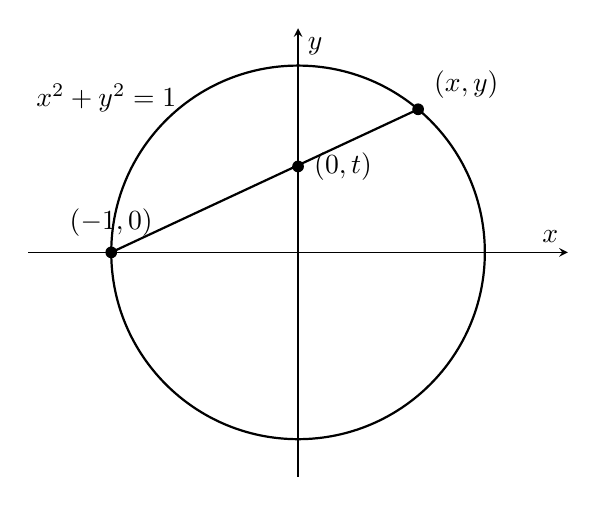
\begin{tikzpicture}
\begin{axis}[axis equal,axis lines=middle,xmin=-1.2,xmax=1.2,ymin=-1.2,ymax=1.2,xtick=\empty,ytick=\empty,xlabel=$x$,ylabel=$y$]
\draw[thick] (-1,0) -- (0.6427876,0.766);
\draw[thick] (0,0) circle[radius=1];
\draw (-0.6,0.7) node[anchor=south east] {$x^2+y^2=1$};
\node[circle,fill,inner sep=1.5pt,label={90:{$(-1,0)$}}] at (-1,0) {};
\node[circle,fill,inner sep=1.5pt,label={10:{$(x,y)$}}] at (0.6427876,0.766) {};
\node[circle,fill,inner sep=1.5pt,label={0:{$(0,t)$}}] at (0,0.46) {};
\end{axis}
\end{tikzpicture}
\end{center}
\end{example}

\begin{defn}
An \textit{ideal} $I\unlhd R$ of a ring $R$ is a subset of $R$ such that $a,b\in I,r\in R\implies a+b,ar\in I$. For $X\subset R$, denote by $I(X)$ the ideal generated by $X$ (the smallest ideal containing $X$). If $X=\{r_1,\ldots,r_n\}$ one also writes $I(X)=\la r_1,\ldots,r_n\ra$.
\end{defn}

\begin{thm}[Hilbert basis theorem]
\label{thm:Hilbertbasis}
If $R$ is a Noetherian ring then $R[x]$ is also Noetherian, i.e. any ideal in $R[x]$ is finitely generated if any ideal in $R$ is finitely generated.
\end{thm}

\begin{coro}
For a field $\K$, any $I\unlhd\K[x_1,\ldots,x_n]$ has a finite generating set.
\end{coro}

\begin{notation}
$\V_\K(I)=\{(a_1,\ldots,a_n):f(a_1,\ldots,a_n)=0 \ \forall f\in I\}$.
\end{notation}
\begin{remark}
By corollary above, one can write $I=\la f_1,\ldots,f_m\ra$. We claim $\V_\K(I)=\V_\K(f_1,\ldots, f_m)$. Indeed, $\{f_1,\ldots,f_m\}\subset I$ so clearly $\V_\K(I)\subset\V_\K(f_1,\ldots,f_m)$. But for any $g\in I$ one can write $g=g_1f_1+\cdots+g_mf_m$, so $\V_\K(I)\supset\V_\K(f_1,\ldots,f_m)$ as well.
\end{remark}

\begin{flushright}
\textit{Week 2, lecture 1, 7th October}
\end{flushright}

\begin{defn}
Define the \textit{Zariski topology} by: a set $V\subset\K^n$ is closed $\iff V$ is an affine algebraic set.
\end{defn}

\begin{remark}
\label{remark:Zariskitopology}
The Zariski topology is indeed a topology: $\K^n=\V_\K(0),\varnothing=\V=\K(1)$, intersection of arbitrary closed sets is closed by \ref{thm:Hilbertbasis} ($\V_\K(f_1,\ldots,f_n)\cap\V_\K(g_1,\ldots,g_m)=\V_\K(f_1,\ldots,f_n,g_1,\ldots,g_m)$), and finite union of closed sets is close ($\V_\K(f_1,\ldots,f_m)\cup\V_\K(g_1,\ldots,g_m)=\V_\K(\prod_{i,j}f_ig_j$).

Note that Zariski topology is coarser (weaker) than the usual Euclidean topology since any polynomial is a continuous function, and closedness is preserved under preimage, but e.g. $[a,b]\subset\R$ is closed with respect to Euclidean norm, but not an affine algebraic set.
\end{remark}

\begin{defn}
A field $\K$ is \textit{algebraically closed} if $f\in\K[x]\implies \exists a\in\K:f(a)=0$.
\end{defn}

\begin{thm}[Fundamental theorem of algebra]
$\C$ is algebraically closed.
\end{thm}

\begin{lemma}
\label{lemma:algclosedfieldisinfinite}
An algebraically closed field must be infinite.
\end{lemma}
\begin{proof}
Suppose $\K$ is a finite field, then $f(x)=\prod_{a\in\K}(x-a)+1$ has no roots in $\K$.
\end{proof}

\begin{thm}
\label{thm:curveshaveinfpoints}
If $\K$ is algebraically closed, then any plane curve $C\subset\K^2$ has infinitely many points.
\end{thm}
\begin{proof}
Let $C=\V_\K(p)$ be a plane curve and consider $p\in\K[x,y]=\K[y][x]$ as
\[
Q_d(y)x^d+\cdots+Q_1(y)x+Q_0(y)
\]
where WLOG $d\geq 1$ and $Q_i(y)\in\K[y]$. Now $Q_d(y)$ has at most $\deg_y Q_d$ roots, so since $\K$ is infinite by \ref{lemma:algclosedfieldisinfinite}, there are infinitely many $y_0:Q_d(y_0)\neq 0\implies \deg p=d$. But again $\K$ is algebraically closed, hence for every such $y_0,\ \exists x_0:p(x_0,y_0)=0$.
\end{proof}

\subsection{Factorisation}
\begin{defn}
An \textit{integral domain} or \textit{domain} is a ring where product of any two nonzero elements is nonzero.

An element $a\in R$ of a ring is a \textit{unit} if $\exists a^{-1}:a^{-1}a=1$.

A nonzero element $a\in R$ is \textit{irreducible} if it's not a product of two nonunit elements.

A \textit{unique factorisation domain} is a domain $R$ where any nonzero and nonunit element can be written uniquely (up to reordering and multiplication by units) as product of irreducible elements.
\end{defn}

\begin{thm}
If $R$ is a UFD, then $R[x]$ is a UFD.
\end{thm}
\begin{proof}
See MATH70035 Algebra 3.
\end{proof}

\begin{coro}
\label{coro:KfieldKxUFD}
If $\K$ is a field, then $\K[x_1,\ldots,x_n]$ is a UFD.
\end{coro}

\begin{thm}[Weak Nullstellensatz]
\label{thm:weak0stellensatz}
If $\K$ is algebraically closed and $I\unlhd\K[x_1,\ldots,x_n]$, then
\[
\V_\K(I)=\varnothing\iff 1\in I\iff I=\K[x_1,\ldots,x_n].
\]
\end{thm}
\begin{proof}
Let $m=\la x1-a_1,\ldots,x_n-an\ra\unlhd\K[x_1,\ldots,x_n]$ be a maximal ideal which has $\V_\K(m)=\{(a_1,\ldots,a_n)\}$. But then for any ideal $I$ other than $\K$ one has $I\subset m$, so $\V_\K(m)\subset\V_\K(I)$, in particular $\V_\K(I)\neq\varnothing$.
\end{proof}

\begin{coro}
\label{coro:fdivgthenVfinVg}
If $f,g\in \K[x_1,\ldots,x_n]$ then $f\mid g\implies \V_\K(f)\subset\V_\K(g)$.
\end{coro}

\begin{prop}[The converse]
\label{prop:VfinVgthenfdivg}
Let $\K$ be algebraically closed and $f,g\in\K[x_1,\ldots,x_n]$. If $f$ is irreducible and $\V_\K(f)\subset\V_\K(g)$ then $f\mid g$.
\end{prop}
\begin{proof}
$\V_\K(f)\subset\V_\K(g)\iff\{f=0\}\cap\{g\neq 0\}=\varnothing$, but $g(x_1,\ldots,x_n)\neq 0\iff\exists t\in\K:tg(x_1,\ldots,x_n)=1$ (any nonzero element of a field is a unit), so one has $\V_\K(f)\cap\V_\K(tg-1)=\V_\K(f,tg-1)=\varnothing$ where $tg-1\in\K[x_1,\ldots,x_n,t]$. By \ref{thm:weak0stellensatz}, $1\in\la f,tg-1\ra$, i.e. $af+b(tg-1)=1$ for some $a,b\in\K[x_1,\ldots,x_n,t]$. Now write $t=\frac1g$ and multiply the above by $g^N$ where $N$ is large enough so that $\widetilde a f=g^N$ where $\widetilde a\in\K[x_1,\ldots,x_n]$. In particular $f\mid g^N$, but $f$ is irreducible, so since $\K[x_1,\ldots,x_n]$ is a UFD by \ref{coro:KfieldKxUFD} $f$ is prime, hence $f\mid g$.
\end{proof}

\begin{flushright}
\textit{Week 2, lecture 2, 7th October}
\end{flushright}

\begin{defn}
\label{defn:irred}
A topological space $X$ is \textit{irreducible} if for any two closed subsets $A,B\subset X$,
\[
X=A\cup B\implies X=A\text{ or }X=B.
\]

An affine algebraic set $\V\subset\K^n$ is \textit{reducible} if one can write $\V=\V_1\cup\V_2$ where $V_i$'s are affine algebraic and $V_i\neq V$. Otherwise it's \textit{irreducible}, i.e. if $\V=\V_1\cup\V_2\implies \V=\V_1$ or $\V_2$.
\end{defn}

\begin{thm}
\label{thm:CisirrediffCisVKfwirredf}
Let $\K$ be algebraically closed. Then a plane curve $C\subset\K^2$ is irreducible $\iff C=\V_\K(f)$ for some nonconstant irreducible $f\in\K[x,y]$.
\end{thm}
\begin{proof}
Let $C=\V_\K(f)$ be irreducible and write $f=f_1^{\alpha_1}\cdots f_n^{\alpha_n}$ where $f_i$'s are irreducible. Then
\[
C=\V_\K(f_1)\cup\cdots\cup\V_\K(f_n).
\]
By definition, $\exists i:C=\V_\K(f_i)$.

Now let $C=\V_\K(p)$ where $p$ is irreducible and suppose for a contradiction that $C$ is reducible, i.e.
\[
\exists p_1,p_2:\V_\K(p)=\V_\K(p_1)\cup\V_\K(p_2)=\V_\K(p_1p_2).
\]
But by \ref{prop:VfinVgthenfdivg}, $p\mid p_1p_2$, so WLOG $p\mid p_1$, so by \ref{coro:fdivgthenVfinVg} $\V_\K(p)\subset\V_\K(p_1)\subset\V_\K(p)$, hence $\V_\K(p)=\V_\K(p_1)$, i.e. $C$ is irreducible.
\end{proof}

\begin{thm}
For any affine algebraic set $\V\subset\K^n$, there are unique irreducible affine algebraic sets $\V_1,\ldots,\V_k:\V=\bigcup_{i=1}^k\V_i$ and $\V_i\not\subset\V_j \ \forall i\neq j$. The $\V_i$'s are called \textit{irreducible components} of $\V$.
\end{thm}
\begin{proof}
For existence, we prove that the set
\[
\mathcal F:=\{\text{affine algebraic sets }\V\subset\K^n:\V\text{ is not the union of a finite number of irreducible affine algebraic sets}\}
\]
is empty. For a contradiction, suppose $\V\in\mathcal F$ and it's minimal with respect to inclusion. First note that $\V$ is reducible, so one can write $\V=\V_1\cup\V_2$ where $\V_1,\V_2$ are affine algebraic, but then $\V_1,\V_2\subset\V$ so by assumption $\V_1,\V_2\notin\mathcal \F$, i.e. $\V_1=\cup_i\V_{1i},\V_2=\cup_j\V_{2j}$, but then $\V$ is union of these.

For the condition $\V_i\not\subset\V_j \ \forall i\neq j$ one simply needs to remove the redundant components by inclusion. It remains to show that two decompositions are the same up to reordering. Write
\[
\V=\V_1\cup\cdots\cup\V_k=\W_1\cup\cdots\W_{k'}
\]
then
\[
\V_i=(\V_i\cap\W_1)\cup\cdots\cup(\V_i\cap\W_{k'})
\]
which is irreducible, so $\V_i=\V_i\cap\W_{j(i)}$ for some $j(i)$, i.e. $\V_i\subset\W_{j(i)}$. But the argument is symmetrical, so $\W_{j(i)}\subset\V_k$ for some $k$, but since we got rid of redundant components, it must be $\V_i=\V_k$ and in particular $\V_i=\W_{j(i)}$.
\end{proof}

\begin{coro}
\label{coro:factorsofcurve}
Write $p=p_1^{d_1}\cdots p_n^{d_n}\in\K[x,y]$ where $p_i$ are irreducible and $\C=\V_\K(p)$, then 
\begin{enumerate}
\item $C=\V_\K(p_1)\cup\cdots\cup\V_\K(p_n)$, and
\item if $C=C_1\cup\cdots\cup C_k$ is the irreducible decomposition of $C$, then (up to reordering) $C_i=\V_\K(p_i)$ and $k=n$.
\end{enumerate}
\end{coro}

\begin{coro}
\label{coro:fgsharezerosifffislg}
If each of the irreducible decompositions of $f,g\in\K[x,y]$ has no repeated factors, then $\V_\K(f)=\V_\K(g)\iff f=\lambda g$ for some $\lambda\in\K$.
\end{coro}

\begin{flushright}
\textit{Week 2, lecture 3, 11th October}
\end{flushright}

\section{Projective variety}
\subsection{Motivation, definitions, basic results}
The motivation to define projective things is we want things to be compact (in the usual Euclidean topology): consider intersection of curves $y^2=x^2+1$ and $y=\alpha x$. If $\alpha\neq\pm 1$ one always has exactly two intersections, but if $\alpha=\pm 1$ the line is asymptotic so we don't have intersection -- that is, if we don't consider points at infinity.

\begin{center}
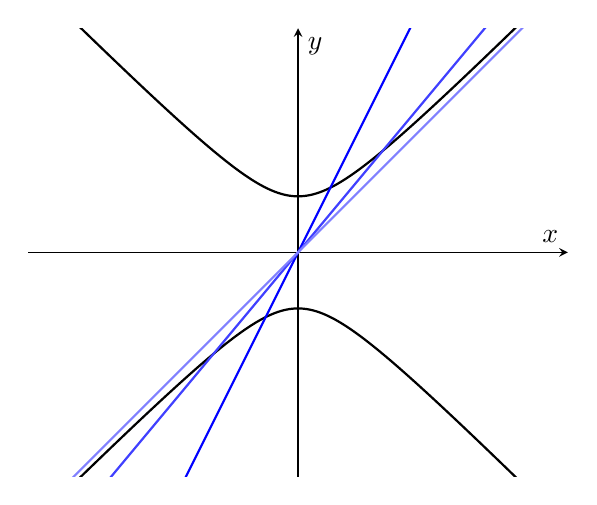
\begin{tikzpicture}
\begin{axis}[axis equal,axis lines=middle,xmin=-1,xmax=1,ymin=-4,ymax=4,xtick=\empty,ytick=\empty,xlabel=$x$,ylabel=$y$]
\addplot[smooth,samples=100,no markers,thick] {sqrt(x^2+1)};
\addplot[smooth,samples=100,no markers,thick] {-sqrt(x^2+1)};
\addplot[smooth,samples=100,no markers,thick,blue] {2*x};
\addplot[smooth,samples=100,no markers,thick,blue!75] {1.2*x};
\addplot[smooth,samples=100,no markers,thick,blue!50] {x};
\end{axis}
\end{tikzpicture}
\end{center}

But how do we formalise ``points at infinity''? That's where the word ``projective'' comes in.

\begin{center}
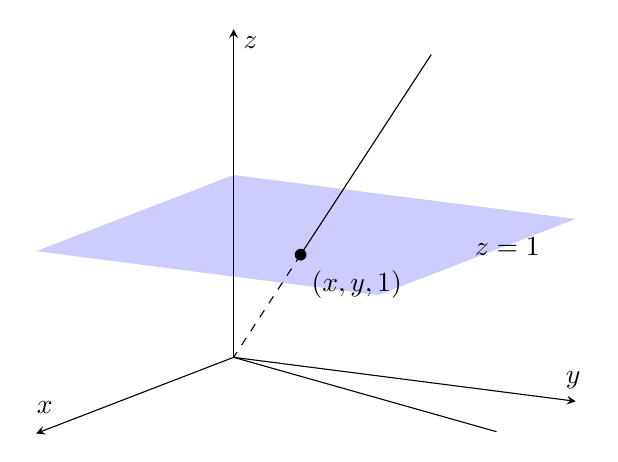
\begin{tikzpicture}
\begin{axis}[axis lines=middle,xmin=0,xmax=1,ymin=0,ymax=1,zmin=0,zmax=1.8,view={120}{15},xtick=\empty,ytick=\empty,ztick=\empty,xlabel=$x$,ylabel=$y$,zlabel=$z$]
\fill[name path=toppath, blue, fill opacity=0.2] (axis cs:1,0,1) -- (axis cs:1,1,1) -- (axis cs:0,1,1) -- (axis cs:0,0,1) -- cycle;
\node[circle,fill,inner sep=1.5pt,label={280:{$(x,y,1)$}}] at (0.7,0.6,1) {};
\draw[dashed] (0.7,0.6,1) -- (0,0,0);
\node at (0,0.8,0.8) {$z=1$};
\draw (0.7,0.6,1) -- (2.1,1.8,3);
\draw (0,0,0) -- (0.4,1,0);
\end{axis}
\end{tikzpicture}
\end{center}

For any point $(x,y)\in\K^2$, one can ``project'' it to the $z=1$ plane to get a unique point $(x,y,1)$ in the way shown above. One then consider points as lines, more specifically 1-dimensional subspaces. The points at infinity have $z$-coordinate 0, i.e. the line connecting origin and the projected point is entirely in the $xy$-plane so they don't reach the $z=1$ plane.

\begin{defn}
The $n$-dimensional \textit{projective space}, denoted by $\p^n$ (or more specifically $\p^n(\K)$) is $\K^{n+1}\backslash\{0\}$ modulo the equivalence relation $p\sim q\iff p=\lambda q$ for some $\lambda\in\K$. An element of $\p^n$ is written as $[x_0,\ldots,x_n]$, which is the equivalence class for $(x_0,\ldots,x_n)$.

One equips $\p^n$ with the quotient topology: $U\subset\p^n$ is open if $\{x\in\K^{n+1}\backslash\{0\}:x\sim u\text{ for some }u\in U\}$ is open.
\end{defn}
\begin{example}
\label{example:understandPn}
$\p^0$ is a point, $\p^1$ can be understood as $\K\cup\p^0$ (the lines $y=ax$ where $a$ is allowed to be $\infty$ (the $y$-axis)).
\end{example}

\begin{remark}
\label{remark:charts}
We claim $U_j:=\{[x_0,\ldots,x_n]:x_j\neq 0\}\subset\p^n$ (the \textit{affine charts} in manifold language) is homeomorphic to $\K^n$. The map $\varphi$ defined by
\[
\begin{aligned}
\varphi&:U_j\rightarrow\K^n:[x_0,\ldots,x_n]\mapsto\left(\frac{x_0}{x_j},\ldots,\frac{x_{j-1}}{x_j},\frac{x_{j+1}}{x_j},\ldots,\frac{x_n}{x_j}\right) \\
\varphi^{-1}&:\K^n\rightarrow U_j:(y_1,\ldots,y_n)\mapsto [y_1,\ldots,y_j,1,y_{j+1},\ldots,y_n]
\end{aligned}
\]
is indeed bijective, and since $\p^n$ is equipped with quotient topology inherited from $\K^{n+1}\supset\K^n$ one has that $\varphi$ preserves open sets as well, i.e. it's homeomorphic.

Now note that $\p^n=\bigcup_{j=0}^n U_j$, so one can understand $\p^n$ as $n+1$ copies of $\K^n$. One can also think of $\p^n$ as $\K^n\cup\p^{n-1}$, where $\K^n$ corresponds to the $x_n\neq 0$ part and $\p^{n-1}$ corresponds to the $x_n=0$ part (see image above).
\end{remark}

\begin{remark}
\label{remark:PnCiscompact}
Let $\K=\C$. Define
\[
S^{2n+1}:=\{(x_0,\ldots,x_n)\in\C^{n+1}\cong\R^{2n+2}:|x_0|^2+\cdots+|x_n|^2=1\}
\]
and
\[
\pi:S^{2n+1}\rightarrow\p^n(\C):(x_0,\ldots,x_n)\mapsto [x_0,\ldots,x_n].
\]
The preimage of $[x_0,\ldots,x_n]$ is then $\{(\lambda x_0,\ldots,\lambda x_n) \in S^{2n+1}\}$.

The map is clearly surjective and, similar to previous remark, continuous. We've shown $\p^n(\C)$ is compact since $S^{2n+1}$ is compact (closed and bounded) by Heine--Borel. It's also Hausdorff.
\end{remark}

\begin{flushright}
\textit{Week 3, lecture 1, 14th October}
\end{flushright}

To make sense of polynomials over $\p^n$, we need to characterise polynomials satisfying that if $(x_0,\ldots,x_n)$ is a solution then $(\lambda x_0,\ldots,\lambda x_n)$ is also a solution for any $\lambda\in\K$.

\begin{defn}
A polynomial $f\in\K[x_0,\ldots,x_n]$ is \textit{homogeneous} of degree $d$ if
\[
f(\lambda x_0,\ldots,\lambda x_0)=\lambda^d f(x_0,\ldots,x_n) \qquad \forall\lambda\in\K,(x_0,\ldots,x_n)\in\K^{n+1}.
\]
\end{defn}
\begin{remark}
\label{remark:homogeneous}
Observe that monomial $f=cx_0^{e_0}\cdots x_n^{e_n}$ is homogeneous of degree $\sum_{i=0}^n e_i$. We claim any homogeneous polynomial is a sum of monomials of the same degree. Indeed, for any $f\in\K[x_0,\ldots,x_n]$ with degree $d$ one can write $f=f_d+f_{d-1}+\cdots+f_0$ where $f_i$ only contain monomials of degree $i$. Then $f$ is homogeneous of degree $d\iff f=f_d$. It's clear that $f=f_d\implies f$ is homogeneous by the observation. Now if $f$ is homogeneous then
\[
\begin{aligned}
f(\lambda x_0,\ldots,\lambda x_n)&=\lambda^d f_d(x_0,\ldots,x_n)+\lambda^d f_{d'<d}(x_0,\ldots,x_n) \qquad \text{by definition of homogeneous} \\
&=\lambda^d f_d(x_0,\ldots,x_n)+\lambda^{d-1}f_{d-1}(x_0,\ldots,x_n)+\cdots+\lambda f_1(x_0+\cdots+x_n)+f_0\qquad\text{by calculation,}
\end{aligned}
\]
so it must e $f_{d'<d}=0$.

Also a key observation is that if $p=gh$ is homogeneous then $g,h$ are homogeneous, which can be proved easily by contradiction.
\end{remark}

\begin{lemma}
If $f\in\K[x_0,\ldots,x_n]$ is homogeneous then the set
\[
\{[x_0,\ldots,x_n]\in\p^n:f(x_0,\ldots,x_n)=0\}
\]
is well-defined.
\end{lemma}
\begin{proof}
It suffices to show that the set does not depend the choice of representative $(x_0,\ldots,x_n)$ of $[x_0,\ldots,x_n]$, i.e. if $p\sim q$ and $f(p)=0$ then $f(q)=0$, but this is clear:
\[
f(x_0,\ldots,x_n)=0\implies f(\lambda x_0,\ldots,\lambda x_n)=\lambda^d f(x_0,\ldots,x_n)=\lambda^d 0=0.
\]
\end{proof}

\begin{defn}
A \textit{projective variety} is a set $\V\subset\p^n(\K)$ that can be written as
\[
\V=\{[x_0,\ldots,x_n]\in\p^n:f_1(x_0,\ldots,x_n)=\cdots=f_k(x_0,\ldots,x_n)=0\}
\]
where $f_i$'s are homogeneous.
\end{defn}

\begin{prop}
Let $\K$ be algebraically closed and $f\in\K[x,y]$ homogeneous of degree $d$, then one can write $f(x,y)=\prod_{i=1}^d (a_ix+b_iy)$ where $a_i,b_i$ not both 0, and $\p^1\supset\V(f)=\{[-b_1,a_1],\ldots,[-b_d,a_d]\}$.
\end{prop}
\begin{proof}
Write $f=y^{d-e}g(x,y)$ where $g$ is homogeneous of degree $e$ and $y\nmid g(x,y)$. Write
\[
\begin{aligned}
g(x,y)&=c_ex^e+c_{e-1}x^{e-1}y+\cdots+c_0y^e\qquad\text{where }c_e\neq 0 \\
&=y^e c_e\left(\left(\frac{x}{y}\right)^e+\frac{c_{e-1}}{c_e}\left(\frac{x}{y}\right)^{e-1}+\cdots+\frac{c_0}{c_e}\right)\\
&=y^e c_e \prod_{i=1}^e\left(\frac{x}{y}-t_i\right) \qquad\text{for some }t_i\in\K\text{ since }\K\text{ is algebraically closed} \\
&=c_e\prod_{i=1}^e(x-t_iy).
\end{aligned}
\]
\end{proof}

So projective varieties in $\p^1$ are not so interesting after all. To have curves we need to go one dimension higher.

\begin{defn}
A \textit{projective plane curve} of degree $d>0$ is a set of the form
\[
C=\{[x_0,x_1,x_2]\in\p^2:p(x_0,x_1,x_2)=0\}
\]
where $p$ is nonconstant and homogeneous of degree $d$.
\end{defn}

\begin{flushright}
\textit{Week 3, lecture 2, 14th October}
\end{flushright}

One can define irreducibility similar for projective plane curves to \ref{defn:irred} and analogously one has:

\begin{prop}
\label{prop:4resultsofppc}
If $\K$ is algebraically closed and $C\subset\p^2(\K)$ is a projective plane curve, then
\begin{enumerate}
\item $C$ has infinitely many points. (cf. \ref{thm:curveshaveinfpoints})
\item $C$ is irreducible $\iff C=\{p=0\}$ for some irreducible homogeneous polynomial $p$. (cf. \ref{thm:CisirrediffCisVKfwirredf})
\item If $p,q\in\K[x,y,z]$ are irreducible homogeneous polynomials, then $\{p=0\}=\{q=0\}\iff p=\lambda q$ for some $\lambda\in\K$ (cf. \ref{coro:fgsharezerosifffislg})
\item If $p=p_1^{\alpha_1}\cdots p_k^{\alpha_k}$ where $p_i$'s are irreducible, then the irreducible components of $C=\{p=0\}$ are precisely $\{p_i=0\}$. (cf. \ref{coro:factorsofcurve})
\end{enumerate}
\end{prop}

\begin{prop}
Let $C\subset\p^2(\C)$ be a projective plane curve. Then $C$ is compact.

This is the key motivation/expectation when we defined projective spaces.
\end{prop}
\begin{proof}
$\p^2(\C)$ is compact by \ref{remark:PnCiscompact}, and $C\subset\p^2(\C)$ is closed since its preimage in $\C^3\backslash\{0\}$ with respect to the natural quotient map is closed (since it's a preimage of a closed set of a continuous function, see \ref{remark:Zariskitopology}), but any closed subset of a compact space is compact.
\end{proof}

\subsection{Projective plane curves -- affine plane curves}
Again, per \ref{remark:charts}, consider $\p^2$ as $\{x\neq 0\}\cup\{y\neq 0\}\cup\{z\neq 0\}$, and every point $(x,y)\in\K^2$ corresponds uniquely to the point $[x,y,1]$ in $\p^2$, i.e. the unique point where the line defined by $(0,0,0)$ and $(x,y,1)$ intersects with the $z=1$ plane.

For a projective plane curve $\overline C=\{p(x,y,z)=0\}$ where $z\nmid p$ (i.e. the line $\{z=0\}$ (the ``line at infinity'', denoted by $L_\infty$) is not fully contained in $\overline C$), one can map it to an affine plane curve $C=\{p(x,y,1)=0\}\in\K^2$ where now $p\in\K[x,y]$ (since $z\nmid p$, one can make sure this $p$ is nonconstant).

\begin{example}
The projective plane curve $\overline C=\{xy+z^2=0\}$ corresponds to $C=\{xy+1=0\}\subset\K^2$, so it's a hyperbola. But it also has points at infinity, i.e. $\overline C\cap L_\infty=\{xy=0\}=\{[1,0,0],[0,1,0]\}$.
\end{example}

How does one map an affine plane curve to a projective one? First note that $f$ may not be homogeneous so one needs to homogenize it, and also a polynomial over $\p^2$ has three variables so we need to add one more. We can do both at the same time.

\begin{lemma}
If $f\in\K[x,y]$ is of degree $d$, then its \textit{homogenization} $F(x,y,z):=z^d f\left(\frac{x}{z},\frac{y}{z}\right)$ is homogeneous of degree $d$ such that $F(x,y,1)=f(x,y)$ and $z\nmid F$.
\end{lemma}
\begin{proof}
Any monomial in $f$ is of the form $cx^iy^j$ where $i+j\leq d$, which is homogenized to $z^d c\left(\frac{x}{z}\right)^i\left(\frac{y}{z}\right)^j=cz^{d-i-j}x^iy^j$, indeed a monomial in $\K[x,y,z]$ with degree $d-i-j+i+j=d$. Since $\deg f=d$, there is a homogenized monomial $cx^iy^j$ where $i+j=d$, so $z\nmid F$.
\end{proof}

We can now map $C=\{0=f\in\K[x,y]\}\subset\K^2$ to $\overline C=\{F[x,y,z]=0\}$ where $F$ is the homogenization of $f$. We claim
\begin{thm}
The map
\[
\begin{aligned}
\phi:\{\text{projective plane curves not containing }\{z=0\}\}&\rightarrow\{\text{affine plane curves}\} \\
\overline C=\{p(x,y,z)=0\}\subset\p^2(\K)&\mapsto C=\{p(x,y,1)=0\}\subset\K^2
\end{aligned}
\]
is bijective with the inverse
\[
\begin{aligned}
\psi:\{\text{affine plane curves}\}&\rightarrow\{\text{projective plane curves not containing }\{z=0\}\} \\
C=\{f(x,y)=0\}\subset\K^2&\mapsto\overline C=\{F(x,y,z)=0\}\subset\p^2(\K)
\end{aligned}
\]
\end{thm}
\begin{proof}
It suffices to see that $F(x,y,1)=f(x,y)$ which follows from the lemma above.
\end{proof}
Of course this bijection is not unique, we chose in particular the $z=1$ hyperplane.

\begin{flushright}
\textit{Week 3, lecture 3, 18th October: example/exercise class}
\end{flushright}

\begin{flushright}
\textit{Week 4, lecture 1, 21st October}
\end{flushright}

We mentioned ``points at infinity'' many times and let's now formalise it.
\begin{defn}
Let $C$ be an affine plane curve. The \textit{points at infinity} of $C$ is the set $\overline C\cap L_\infty$.
\end{defn}

\begin{prop}
There is a bijection
\[
\begin{aligned}
\overline C\cap L_\infty &\leftrightarrow \{[x,y]\in\p^1:f_d(x,y)=0\} \\
[x,y,0]&\mapsto [x,y]
\end{aligned}
\]
\end{prop}
where $f_d$ is the homogeneous of degree $d$ part of $f$.
\begin{proof}
Let $C=\{f(x,y)=0\}\subset\K^2$ where $\deg f=d$. Then one can write $f=f_d+f_{d-1}+\cdots+f_0$ where each $f_i$ is homogeneous of degree $i$. Then
\[
F(x,y,z)=f_d(x,y)+zf_{d-1}(x,y)+\cdots+z^df_0(x,y).
\]
Hence
\[
\overline C\cap L_\infty=\{F(x,y,z)=0\}\cap\{z=0\}=\{F(x,y,0)=0\}=\{[x,y,0]:f_d(x,y)=0\}.
\]
\end{proof}
\begin{example}
Consider $C=\V_\K(f)$ where $f(x,y)=x^3+xy^2+xy+\cdots$. Then
\[
\overline C\cap L_\infty=\{[x,y,0]\in\p^1:x^3+xy^2=0\}=\{[0,1,0],[i,-1,0],[i,1,0]\}.
\]
\end{example}

From now on we assume our polynomials have no repeated factors, i.e. if $F=f_1^{\alpha_1}\cdots f_n^{\alpha_n}$ where each $f_i$ is irreducible then each $\alpha_i=1$.

\subsection{Singular point, smooth curve}
Recall in real analysis one has
\begin{thm}[Special case of implicit function theorem]
Let $F:\R^2\rightarrow\R$ be a smooth (i.e. infinitely differentiable) function with $F(a,b)=0$ and $\frac{\partial F}{\partial y}(a,b)\neq 0$. Then $\exists \delta,\varepsilon>0$ such that $\forall x$ in the box
\[
\beta=\{(x,y)\in\R^2:|x-a|<\delta,|y-b|<\varepsilon\}
\]
$\exists! y$ in the box such that $F(x,y)=0$.

This correspondence gives a smooth function $f$ over $|x-a|<\delta$ such that $F(x,y)=0$ for $(x,y)\in\beta\iff y=f(x)$. In plain English, the theorem says a smooth curve is locally the graph of a smooth function.
\end{thm}
\begin{proof}
WLOG assume $\frac{\partial F}{\partial y}(a,b)>0$. Than $F$ is increasing in $y$ in a small enough neighbourhood of $(a,b)$, i.e. $\exists\delta_1,\varepsilon_1>0:\frac{\partial F}{\partial y}(x,y)>0 \ \forall x,y:|x-a|<\delta_1,|y-b|<\varepsilon_1$. Hence by continuity of $F$,
\[
\exists\delta,\varepsilon:|x-a|<\delta\implies F(x,b+\varepsilon)>0
\]
and $F(x,b-\varepsilon)<0$. But then the intermediate value theorem says $\forall x:|x-a|<\delta,\ \exists!y:|y-b|<\varepsilon$ and $F(x,y)=0$.
\end{proof}

\begin{defn}
Let $C=\{f(x,y)=0\}\subset\K^2$ be an affine plane curve. $C$ is \textit{smooth} at $(a,b)\in C$ if
\[
\left(\frac{\partial f}{\partial x}(a,b),\frac{\partial f}{\partial y}(a,b)\right)\neq (0,0).
\]
Otherwise the point is \textit{singular}, or a \textit{singularity}.

One can therefore write the down the set of singular points of $C=\V_\K(f)$ as $\V_\K\left(f,\frac{\partial f}{\partial x},\frac{\partial f}{\partial y}\right)$.

$C$ is a \textit{smooth curve} if $C$ is smooth at every $(a,b)\in C$.

For a smooth point $p\in C$, one can define its \textit{tangent line} by
\[
T_pC=\left\{\frac{\partial f}{\partial x}(a,b)(x-a)+\frac{\partial f}{\partial y}(a,b)(y-b)=0\right\}
\]
\end{defn}
\begin{example}
Any affine line $\V_\K(f=ax+by+c)$ is smooth; since $ax+by+c$ is nonconstant, either $a=\frac{\partial f}{\partial x}$ or $b=\frac{\partial f}{\partial y}$ is nonzero.
\end{example}

\begin{defn}
A \textit{nodal} singularity is where two smooth irreducible components intersect. We'll later see a proof of why we don't have to specify anything about partial derivatives.
\end{defn}
\begin{example}
The curve $\{xy=0\}=\{x=0\}\cup\{y=0\}$ has a nodal singularity at $(0,0)$.
\end{example}

\begin{flushright}
\textit{Week 4, lecture 2, 21st October}
\end{flushright}

\begin{minipage}{0.75\textwidth}
\begin{defn}
A \textit{cusp} singularity is a sharp point of a curve where there's a sudden change in direction.
\end{defn}
\begin{example}
The curve $C=\{f=y^2-x^3=0\}$ has a singularity where
\[
\frac{\partial f}{\partial x}=3x^2=\frac{\partial f}{\partial y}=2y=y^2-x^3=0,
\]
so $(0,0)$ is singular, which is a cusp as evident on the right.
\end{example}
\end{minipage}
\begin{minipage}{0.25\textwidth}
\begin{tikzpicture}[scale=0.6]
\begin{axis}[axis lines=middle,xmin=-0.5,xmax=3,ymin=-3,ymax=3,xtick=\empty,ytick=\empty,ztick=\empty,xlabel=$x$,ylabel=$y$]
\addplot[smooth,samples=1000,no markers,thick] {sqrt(x^3)};
\addplot[smooth,samples=1000,no markers,thick] {-sqrt(x^3)};
\node[circle,fill,inner sep=1.5pt] at (0,0) {};
\end{axis}
\end{tikzpicture}
\end{minipage}

\begin{minipage}{0.75\textwidth}
\begin{example}
The \textit{elliptic} curve $C=\{y^2-x^3+x=0\}$ has singularity where
\[
\frac{\partial f}{\partial x}=-3x^2+1=\frac{\partial f}{\partial y}=2y=y^2-x^3+x=0,
\]
which has no solutions, hence $C$ is smooth. 
\end{example}
\end{minipage}
\begin{minipage}{0.25\textwidth}
\begin{tikzpicture}[scale=0.6]
\begin{axis}[axis lines=middle,xmin=-1.5,xmax=2.5,ymin=-2,ymax=2,xtick=\empty,ytick=\empty,xlabel=$x$,ylabel=$y$]
\addplot[smooth,thick] table {data.dat};
\end{axis}
\end{tikzpicture}
\end{minipage}

\begin{remark}
Suppose $f=g^2h\in\K[x,y]$. Then by chain rule and product rule
\[
\frac{\partial f}{\partial x}=2gh\frac{\partial g}{\partial x}+g^2\frac{\partial h}{\partial x}, \qquad \frac{\partial f}{\partial y}=2gh\frac{\partial g}{\partial y}+g^2\frac{\partial h}{\partial y},
\]
so $\{g=0\}\subset\{\text{singularities of }f\}$, but then every point of $\{f=0\}$ is singular, a strange behaviour. This is why we are assuming our polynomials have no repeated factors.
\end{remark}

\begin{defn}
Suppose $\Char\K=0$. A projective plane curve $C=\{F(x,y,z)=0\}\subset\p^2(\K)$ is \textit{singular} at $[a,b,c]$ if
\[
\frac{\partial F}{\partial x}(a,b,c)=\frac{\partial F}{\partial y}(a,b,c)=\frac{\partial F}{\partial z}(a,b,c)=0.
\]
Otherwise the point is \textit{smooth}.
\end{defn}

\begin{example}
$C=\{F=x^d+y^d+z^d=0\}\subset\p^2$ is smooth since $\frac{\partial F}{\partial x}=\frac{\partial F}{\partial y}=\frac{\partial F}{\partial z}=0$ only at $(0,0,0)$, but this is not a point in $\p^2$.
\end{example}

Note that unlike the affine case, we didn't have to specify that $[a,b,c]\in C$, since $\Char\K=0$ implies that as long as the partial derivatives are zero, the point automatically lies on the curve:
\begin{prop}[Euler's identity]
\label{prop:eulersid}
Let $F\in\K[x_0,\ldots,x_n]$ be homogeneous of degree $d$. Then
\[
\sum_{i=0}^n x_i \frac{\partial F}{\partial x_i}=dF.
\]
In particular, if $d\neq 0$ in $\K$ (e.g. if $\Char\K=0$) and $\frac{\partial F}{\partial x_i}(a_0,\ldots,a_n)=0 \ \forall i$, then $F(a_0,\ldots,a_n)=0$.
\end{prop}
\begin{proof}[Proof 1]
It suffices to show for a monomial $F=x_0^{i_0}\cdots x_n^{i_n}$ since a homogeneous polynomial is a sum of monomials of the same degree and one can extend the result linearly. But then
\[
x_0 i_0 x_0^{i_0-1}x_1^{i_1}\cdots x_n^{i_n}+\cdots+x_nx_0\cdots i_nx_n^{i_n-1}=i_0F+\cdots+i_nF=dF
\]
as desired.
\end{proof}
\begin{proof}[Proof 2]
Alternatively, by definition of homogeneous
\[
F(\lambda x_0,\ldots,\lambda x_n)=\lambda^d F(x_0,\ldots,x_n).
\]
Treat $\lambda$ as a variable and differentiate both sides with respect to it:
\[
\sum_{i=0}^n x_i\frac{\partial F}{\partial x_i}(\lambda x_0,\ldots,\lambda x_n)=d\lambda^{d-1}F(x_0,\ldots,x_n),
\]
and setting $\lambda=1$ gives the desired.
\end{proof}

\begin{prop}
Let $\overline C\subset\p^2(\K)$ be the projectivisation of an affine curve $C\subset\K^2$. Then $(a,b)\in C$ is singular $\iff [a,b,1]\in\overline C$ is singular.
\end{prop}
\begin{proof}
Since $f(x,y)=F(x,y,1)$, clearly
\[
\frac{\partial F}{\partial x}(a,b,1)=\frac{\partial f}{\partial x}(a,b)\quad\text{and}\quad\frac{\partial F}{\partial y}(a,b,1)=\frac{\partial f}{\partial y}(a,b),
\]
so $[a,b,1]\in\overline C$ is singular $\implies (a,b)\in C$ is singular. Conversely, if $(a,b)\in C$ is singular, then $[a,b,1]\in\overline C$ and by above $\frac{\partial F}{\partial x}(a,b,1)=\frac{\partial F}{\partial y}(a,b,1)=0$ so by \ref{prop:eulersid}
\[
\frac{\partial F}{\partial z}(a,b,1)=dF(a,b,1)-a\frac{\partial F}{\partial x}(a,b,1)-b\frac{\partial F}{\partial y}(a,b,1)=0.
\]
\end{proof}

One can therefore consider tangent lines (planes in $\K^3$) of projective plane curves:
\[
T_p\overline C=\left\{\frac{\partial F}{\partial x}(a,b,c)(x-a)+\frac{\partial F}{\partial y}(a,b,c)(y-b)+\frac{\partial F}{\partial z}(a,b,c)(z-c)=0\right\},
\]
where the polynomial is indeed homogeneous again by \ref{prop:eulersid}.

\begin{prop}
\label{prop:nodesaresingular}
Let $C$ be a projective plane curve over an algebraically closed field $\K$ and $C_1,C_2$ be two different irreducible components with $[a,b,c]\in C_1\cap C_2$. Then $C$ is singular at $[a,b,c]$. 
\end{prop}
\begin{proof}
By \ref{prop:4resultsofppc}, one can write $C_1=\{f_1=0\},C_2=\{f_2=0\}$ and $f=f_1f_2g$ where $f_1,f_2$ are irreducible. Then
\[
\frac{\partial F}{x_i}=\frac{\partial f_1}{x_i}f_1f_2g+f_1\frac{\partial f_2}{x_i}+f_1f_2\frac{\partial g}{x_i} \quad\forall i
\]
which is 0 at $[a,b,c]$ since $f_1(a,b,c)=f_2(a,b,c)=0$.
\end{proof}
\begin{coro}
\label{coro:smoothimpliesirred}
If $\K$ is algebraically closed, then a smooth projective plane curve must be irreducible.
\end{coro}
This follows from Bézout's theorem, which we will later encounter and prove.

\begin{thm}
Let $C=\{F(x,y,z)=0\}\subset\p^2(\C)$ be a smooth projective plane curve. Then $C$ is a compact Riemann surface (a smooth complex manifold of complex dimension 1).
\end{thm}

\begin{flushright}
\textit{Week 4, lecture 3, 25th October}
\end{flushright}

\section{Bézout theorem}
\subsection{Projective transformation}
\begin{lemma}
For $A\in\GL_{n+1}(\K)$, there is a bijection $\phi_A:\p^n\rightarrow\p^n:[x_0,\ldots,x_n]\mapsto A\begin{bmatrix}x_0\\ \vdots \\ x_n\end{bmatrix}$.
\end{lemma}
\begin{proof}
First $\phi_A$ is well-defined: it's clear that $A\begin{bmatrix}x_0\\ \vdots \\ x_n\end{bmatrix}$ is never zero, and $\phi_A(\lambda p)=\lambda \phi_A(p)\sim\phi_A(p)$. The bijectivity follows immediately from $A$ is invertible.
\end{proof}
\begin{remark}
Note that $\phi_A$ is continuous: a map $f:\p^n\rightarrow X$ is continuous $\iff f\circ\pi:\C^{n+1}\backslash\{0\}\rightarrow X$ is continuous where $\pi:\C^{n+1}\backslash\{0\}\rightarrow\p^n$ is the natural quotient map (which is by definition continuous).
\end{remark}

\begin{defn}
A \textit{projective transformation} $\phi:\p^n\rightarrow\p^n$ is $\phi=\phi_A$ for some $A\in\GL_{n+1}(\K)$, which form the projective general linear group $\PGL_{n+1}$.
\end{defn}
\begin{remark}
Note that $\phi_A=\id_{\p^n}\iff A=\lambda I_{n+1}$, i.e. $\PGL_{n+1}\cong\GL_{n+1}(\K)/\{\lambda I\}$, so one can view $\PGL_{n+1}$ as the group of equivalence classes: $A\sim B\iff A=\lambda B$ for some $\lambda\in\K$.
\end{remark}

\begin{example}[Möbius transformation]
$f:\C\rightarrow\C:z\mapsto\frac{az+b}{cz+d}$ where $ad-bc\neq 0$. One can extend it to infinity: $\overline f(\infty)=\frac{a}{c}$. But $\C\cup\{\infty\}$ is $\p_1$ (recall \ref{example:understandPn}), so $\overline f$ defines a projective transformation $\p^1(\C)\rightarrow\p^1(\C):[x,y]\mapsto\left[ax+by,cx+dy\right]$, where the matrix can be written: $\begin{bmatrix}a&b\\c&d\end{bmatrix}$.
\end{example}

\begin{remark}
There is a explicit Möbius transformation that sends any three distinct points $w_1,w_2,w_3\in\C$ to $0,1,\infty$:
\[
f(z)=\frac{z-w_1}{z-w_3}\frac{w_2-w_3}{w_2-w_1}.
\]
\end{remark}
\begin{lemma}
Given three distinct $w_1,w_2,w_3\in\p_1,\ \exists!$ projective transformation $\phi:w_1\mapsto[0,1],w_2\mapsto[1,1],w_3\mapsto[1,0]$.
\end{lemma}
\begin{proof}
Write $w_i=[a_i,b_i]$ and define
\[
\begin{aligned}
\phi:[x,y]&\mapsto \left[\left(\frac{x}{y}-\frac{a_1}{b_1}\right)\left(\frac{a_2}{b_2}-\frac{a_3}{b_3}\right),\left(\frac{x}{y}-\frac{a_3}{b_3}\right)\left(\frac{a_2}{b_2}-\frac{a_1}{b_1}\right)\right]\\
&=[(b_1x-a_1y)(a_2b_3-a_3b_2),(b_3x-a_3y)(a_2b_1-a_1b_2)]
\end{aligned}
\]
Now suppose $\phi,\phi'$ are two such projective transformations. We want to show $\phi\circ\phi'^{-1}=\lambda I_2$ for some $\lambda\in\K$. Note that $\phi\circ\phi'^{-1}:[0,1]\mapsto [0,1],[1,0]\mapsto [1,0]$ and $[1,1]\mapsto [1,1]$, so the matrix for $\phi\circ\phi'^{-1}$ has eigenvectors $(1,0)$ and $(0,1)$, which means the whole $\K^2$ is the eigenspace.
\end{proof}

\begin{prop}
If no three of $w_1,w_2,w_3,w_4\in\p^2$ are collinear, i.e. writing $w_i=[x_i,y_i,z_i]$ one has
\[
\det\begin{pmatrix}
x_1 & x_2 & x_3 \\ y_1 & y_2 & y_3 \\ z_1 & z_2 & z_3
\end{pmatrix}\neq 0
\](geometrically, the three in points in $\K^3$ are not on the same plane), then $\exists!$ projective transformation $\phi_A:\p^2\rightarrow\p^2:w_1\mapsto [1,0,0],w_2\mapsto [0,1,0],w_3\mapsto [0,0,1],w_4\mapsto [1,1,1]$.
\end{prop}
\begin{proof}
To find this transformation, one first maps an arbitrary $w_4$ to $[1,1,1]$, and then maps $w_1,w_2,w_3$ to $[1,0,0],[0,1,0],[0,0,1]$ in the following way: we first make a map that fixes $[1,0,0],[0,1,0],[0,0,1]$ and sends $[x_4,y_4,z_4]$ to $[1,1,1]$ by the matrix
\[
C=\begin{pmatrix}
\frac{1}{x_4} & 0 & 0 \\
0 & \frac{1}{y_4} & 0 \\
0 & 0 & \frac{1}{z_4}
\end{pmatrix}
\]
(we know $x_4,y_4,z_4\neq 0$ by the linear independency assumption), and clearly the matrix
\[
A=\begin{pmatrix}
x_1 & x_2 & x_3 \\ y_1 & y_2 & y_3 \\ z_1 & z_2 & z_3
\end{pmatrix},
\]
(which we assumed to be invertible) maps $[1,0,0],[0,1,0],[0,0,1]$ to $w_1,w_2,w_3$ respectively, so one needs only to find its inverse and compose it with $C$.
\end{proof}

\begin{flushright}
\textit{Week 5, lecture 1, 28th October}
\end{flushright}

\begin{prop}
Let $C=\{F(x,y,z)=0\}\in\p^2(\K)$ be a projective plane curve and $\phi_A$ a projective transformation. Then
\begin{enumerate}
\item $\phi_A(C)$ is also a projective plane curve.
\item If $C_0$ is an irreducible component of $C$, then $\phi_A(C_0)$ is an irreducible component of $\phi_A(C)$.
\item If $p\in C$ is smooth then $\phi_A(p)\in\phi_A(C)$ is smooth. Moreover, $\phi_A$ preserves the tangent line, i.e.
\[
\phi_A(T_pC)=T_{\phi_A(p)}\phi_A(C).
\]
In particular, if $C$ is smooth then $\phi_A(C)$ is smooth.
\end{enumerate}
\end{prop}
\begin{proof}
Write $B=A^{-1}=(b_{ij})$ and hence $\phi_B=(\phi_A)^{-1}$.
\begin{enumerate}
\item Note that
\[
\begin{aligned}
[x_0,x_1,x_2]\in\phi_A(C) &\iff \phi_B([x_0,x_1,x_2])\in C \\
&\iff \left[\sum_{i=0}^2 b_{0i}x_i,\ldots,\sum_{i=0}^2b_{ni}x_i\right]\in C \\
&\iff F\left(\sum_{i=0}^2 b_{0i}x_i,\ldots,\sum_{i=0}^2b_{ni}x_i\right)=0,
\end{aligned}
\]
so $\phi_A(C)$ is given by the polynomial $G=F\cdot\phi_B$, which is also homogeneous of same degree.
\item It suffices to show that if $C_0$ is irreducible then $\phi_A(C_0)$ is also irreducible since
\[
\phi_A(C)=\phi_A(C_0\cup\cdots\cup C_n)=\phi_A(C_0)\cup\cdot\cup\phi_A(C_n).
\]
Indeed,
\[
\begin{aligned}
x\in \phi_A(C_0\cup\cdots\cup C_n) &\implies \phi_B x\in C_0\cup\cdots\cup C_n \implies \phi_B x\in C_i\text{ for some }i\\
&\implies x\in \phi_A(C_i)\implies x\in\phi_A(C_0)\cup\cdots\cup\phi_A(C_n)
\end{aligned}
\]
If $\phi_A(C_0)=C_1\cup C_2$, then $C_0=\phi_B(C_1)\cup\phi_B(C_2)$, so WLOG $C_0=\phi_B(C_1)$ by assumption, hence $\phi_A(C_0)=C_1$ as desired.
\item Let $p\in\phi_A(C)$ with $\phi_B(p)=q\in C$ smooth. Then by chain rule
\[
\begin{aligned}
\left[\frac{\partial G}{\partial x_0}(p),\frac{\partial G}{\partial x_1}(p),\frac{\partial G}{\partial x_2}(p)\right]&=\left[\frac{\partial F}{\partial x_0}(\phi_B(p)),\frac{\partial F}{\partial x_1}(\phi_B(p)),\frac{\partial F}{\partial x_2}(\phi_B(p))\right]B \\
&=\left[\frac{\partial F}{\partial x_0}(q),\frac{\partial F}{\partial x_1}(q),\frac{\partial F}{\partial x_2}(q)\right]B\neq 0,
\end{aligned}
\]
so $p$ is smooth. Now recall
\[
T_qC=\left\{\frac{\partial F}{\partial x_0}(q)x_0+\frac{\partial F}{\partial x_1}(q)x_1+\frac{\partial F}{\partial x_2}(q)x_2=0\right\},
\]
so
\[
\phi_A(T_qC)=\left\{\frac{\partial F}{\partial x_0}(\phi_Bp)\sum_{i=0}^2 b_{0i}x_i+\frac{\partial F}{\partial x_1}(\phi_Bp)\sum_{i=0}^2 b_{1i}x_i+\frac{\partial F}{\partial x_2}(\phi_Bp)\sum_{i=0}^2 b_{2i}x_i=0\right\}
\]
where the coefficient for $x_i$ is $\frac{\partial G}{\partial x_i}(p)$ again by chain rule.
\end{enumerate}
\end{proof}

\subsection{Resultant}
Let $R$ be a UFD (and so $R[x]$ is a UFD) and $f,g\in R[x]$. We introduce an algebraic tool called resultant to tell us when do $f,g$ have common factors.

\begin{lemma}
If $f,g\in R[x]$ are of degree $d,e\geq 1$ respectively, then $f,g$ have a non-constant common factor $\iff\exists a,b\in R[x]:a,b\neq 0,\ af+bg=0$ with $\deg a\leq e-1,\ \deg b\leq d-1$.
\end{lemma}
\begin{proof}
\begin{itemize}
\item[$\implies$] Suppose $f,g$ have a non-constant common factor and write $f=hq$ and $g=hr$ where $\deg h\geq 1$ (so $\deg q\leq d-1$ and $\deg r\leq e-1$). Then $a=r,b=-q$ satisfy the desired.
\item[$\impliedby$] Write $f=cf_1^{\alpha_1}\cdots f_k^{\alpha_k}$ with $\sum_{i=1}^k\alpha_i=d$. Since $R[x]$ is a UFD, in the factorisation of $bg=-af$ one can find $h=f_1^{\beta_1}\cdots f_k^{\beta_k}$ where $\beta_i\geq\alpha_i \ \forall i$. But then $\deg h=\sum_{i=1}^k\beta_i\geq d$, so $h\nmid b$ and at least some $f_i^{\gamma_i}\mid g$ where $\gamma_i\geq 1$.
\end{itemize}
\end{proof}

\begin{defnthm}
\label{defnthm:resultant}
Another way to formulate the lemma: if one writes the required $a,b$ in the general form: $a(x)=\alpha_{e-1}x^{e-1}+\cdots+\alpha_0,b(x)=\beta_{d-1}x^{d-1}+\cdots+\beta_0$ then $f,g$ have a non-constant common factor if
\[
af+bg=\alpha_{e-1}x^{e-1}f(x)+\cdot+\alpha_0f(x)+\beta_{d-1}\beta^{d-1}g(x)+\cdots+\beta_0g(x)=0
\]
for some $\alpha_{e-1},\ldots,\alpha_0,\beta_{d-1},\ldots,\beta_0\in R$ not all zero, i.e. the $d+e$ polynomials
\[
x^{e-1}f(x),\ldots,f(x),b^{d-1}g(x),\ldots,g(x)
\]
are linearly dependent over $R$. Now write $f(x)=a_dx^d+\cdots+a_0,\ g(x)=b_ex^e+\cdots+b_0$, then if one writes coefficients of the $d+e$ polynomials of maximum $d+e-1$ degree (and hence have $d+e$ coefficients) in rows of a $(d+e)\times (d+e)$ matrix
\[
\begin{pmatrix}
a_d & \cdots & a_0 \\
& a_d & \cdots & a_0 \\
& & \ddots & & \ddots \\
& & & a_d & \cdots & a_0 \\
b_e & \cdots & b_0 \\
& b_e & \cdots & b_0 \\
& & \ddots & & \ddots \\
& & & b_e & \cdots & b_0 \\
\end{pmatrix},
\]
and consider its determinant, called the \textit{resultant} of $f$ and $g$ and denoted by $\re_{f,g}$, then the lemma says: $f,g$ have a non-constant common factor $\iff\re_{f,g}=0$.
\end{defnthm}

\begin{flushright}
\textit{Week 5, lecture 2, 28th October}
\end{flushright}

\begin{example}
An easy example makes it clear: consider $f(x)=x-a,g(x)=x-b\in R[x]$. Then $\deg f=\deg g=1$ so one has a $2\times 2$ matrix with
\[
\re_{f,g}=\det\begin{pmatrix}
1 & -a \\ 1 & -b
\end{pmatrix}=-b+a,
\]
so $f,g$ have a common factor $\iff a=b$.
\end{example}

\begin{prop}
\label{prop:resultant}
If the field of fractions of $R$ has characteristic 0, then $f\in R[x]$ has repeated factors $\iff\re_{f,f'}=0$.
\end{prop}
\begin{proof}
\begin{itemize}
\item[$\implies$] Write $f=g^2h$ where $g,h\in R[x]$ and $\deg g\geq 1$. Then $f'=2gg'h+g^2h'$, so $f,f'$ have the nonconstant common factor $g$, so by \ref{defnthm:resultant} one has $\re_{f,f'}=0$.
\item[$\impliedby$] For any $f$ with $\re_{f,f'}=0$ and an irreducible factor $g$ of $f$, write $f=gh$ and $g\mid f'$. Then $f'=g'h+gh'$, so $g\mid f'-gh'=g'h$. But $\deg g'<\deg g$, so $g\nmid g'$ (one can rule out $g'=0$ since characteristic is 0), hence $g\mid h$ and $g^2\mid f$.
\end{itemize}
\end{proof}

Since this module deals with curves, we are interested in polynomials in more variables.

\begin{prop}
Consider $\K[x,y,z]$ as $\K[y,z][x]$ and let $R=\K[y,z]$. Any homogeneous polynomial $F(x,y,z)$ of degree $d$ can be written as
\[
x^df_0(y,z)+\cdots+f_d(y,z)\in R[x]\qquad\text{where each }f_i\text{ is homogeneous of degree }i.
\]
The leading coefficient is $f_0(y,z)=F(1,0,0)$. To make sure it has the same degree over $\K$ and $R$ as we would expect, assume $F(1,0,0)\neq 0$.

Now similarly write another polynomial $G(x,y,z)$ as $y^eg_0(y,z)+\cdots+g_e(y,z)\in R[x]$ with $g_0(y,z)=G(0,0,1)\neq 0$. Then $\re_{FG}\in R$ is well-defined, and we claim: $\exists A,B\in\K[x,y,z]:\deg_xA\leq e-1,\deg_xB\leq d-1$ and $\re_{F,G}=AF+BG$.

Moreover, if $\re_{F,G}\neq 0$ then it's homogeneous of degree $de$ (as an element of $\K[y,z]$).
\end{prop}
\begin{proof}
Write $\re_{F,G}=\det M$ where $M$ is by definition
\[
\begin{pmatrix}
f_0(y,z) & \cdots & f_d(y,z) \\
& f_0(y,z) & \cdots & f_d(y,z) \\
& & \ddots & & \ddots \\
& & & f_0(y,z) & \cdots & f_d(y,z) \\
g_0(y,z) & \cdots & g_e(y,z) \\
& g_0(y,z) & \cdots & g_e(y,z) \\
& & \ddots & & \ddots \\
& & & g_0(y,z) & \cdots & g_e(y,z) \\
\end{pmatrix}
\]
and do the following column operations to get a new matrix $N$: add $x^{d+e-j}\times$ the $j$th column to the last $d+e$th column for each $j$ from 1 to $d+e-1$. The last column of $N$ is then
\[
\begin{pmatrix}
f_0x^{d+e-1}+\cdots+f_dx^{e-1} \\
\vdots \\
f_0x^d+\cdots+f_d \\
g_0x^{d+e-1}+\cdots+g_ex^{d-1} \\
\vdots \\
g_0x^e+\cdots+g_e
\end{pmatrix}=\begin{pmatrix}
x^{e-1}F\\
\vdots \\
F \\
x^{d-1} G \\
\vdots \\
G
\end{pmatrix}.
\]
Since column operation doesn't change determinant, $\det N=\re_{F,G}$, which is a $R$-linear combination of
\[
x^{e-1}F,\ldots,F,x^{d-1}G,\ldots,G.
\]
This proves $\re_{F,G}=AF+BG$ where $A,B$ satisfy the desired properties.

Now by definition (write $M=(a_{i,j})$)
\[
\re_{F,G}=\det M=\sum_{\sigma\in S_{d+e}}(-1)^\sigma a_{1,\sigma(1)}\cdots a_{d+e,\sigma(d+e)},
\]
and it remains to see each summand $A_\sigma$ is homogeneous of degree $de$. Forget the sign (not relevant considering homogeneity or degree) and split it to two parts: the first $e$ rows (the ones with $f$) and the last $d$ rows (the ones with $g$):
\[
A_\sigma=\prod_{i=1}^e a_{i,\sigma(i)}\prod_{j=e+1}^{d+e} a_{j,\sigma(j)}.
\]
Then for $1\leq i\leq e,\ a_{i,\sigma(i)}=f_{\sigma(i)-i}(y,z)$ which by construction is homogeneous of degree $\sigma(i)-i$, and for $e+1\leq j\leq d+e,\ a_{j,\sigma(j)}=g_{\sigma(j+e)-j}(y,z)$, homogeneous of degree $\sigma(j+e)-j$. So
\[
\begin{aligned}
\deg A_\sigma&=\sum_{i=1}^e (\sigma(i)-i)+\sum_{j=1}^d (\sigma(j+e)-j) \\
&=\sum_{i=1}^{d+e}\sigma(i)-\sum_{i=1}^d i-\sum_{i=1}^e i \\
&=\frac{(d+e)(d+e+1)}{2}-\frac{e(e+1)}{2}-\frac{d(d+1)}{2} \\
&=\frac{d^2+d(e+1)+de}{2}-\frac{d(d+1)}{2} \\
&=\frac{de+de}{2}=de.
\end{aligned}
\]
\end{proof}

\begin{flushright}
\textit{Week 5, lecture 3, 1st November}
\end{flushright}

\begin{coro}
$R_{F,G}$ is the zero polynomial $\iff F$ and $G$ share a nonconstant common factor.
\end{coro}
\begin{proof}
By \ref{prop:resultant}, $R_{F,G}=0\iff F,G$ have a nonconstant common factor as polynomials in $x$, so it remains to ensure that they don't have a common factor that is considered to be ``constant'' in the ring $R=\K[y,z]$. Suppose that $F(x,y,z)=H(y,z)F'(x,y,z)$. But then $F(1,0,0)\neq 0$ and $H(y,z)=0$ (since any factor of a homogeneous polynomial must be homogeneous, recall \ref{remark:homogeneous}), a contradiction.

Conversely it's a more direct application or \ref{prop:resultant}.
\end{proof}

The above discussion about common factors relies on the a priori restrictive condition that $[1,0,0]$ is not on the curves $C_F,C_G$, but this turns out to be not restrictive: we claim that for any $F,G$, one can always find a projective transformation such that $\{F=0\}$ and $\{G=0\}$ do not pass through $[1,0,0]$, by the following lemma.

\begin{lemma}
Let $\K$ be algebraically closed and $C_1,\ldots,C_n\in\p^2(\K)$ projective plane curves. Then $C_1\cup\cdots\cup C_n$ is a proper subset of $\p^2(\K)$.
\end{lemma}
\begin{proof}
If $C_i=\{F_i(X,Y,Z)=0\}$ then $C_1\cup\cdots\cup C_n=\left\{\prod_{i=1}^n F_i(X,Y,Z)=0\right\}$. For a contradiction, suppose $\{x-cy=0\}\subset \left\{\prod_{i=1}^n F_i(X,Y,Z)=0\right\} \ \forall c\in\K$. This would imply $C_1\cup\cdots\cup C_n=\p^2(\K)$. But $\K$ is algebraically closed, so in particular it's infinite, and it's impossible for $\prod_{i=1}^n F_i(X,Y,Z)$ to have infinite irreducible factors, which would follow from our assumption.
\end{proof}

\subsection{Proof and applications of the theorem}
\begin{thm}[Weak Bézout]
\label{thm:weakBezout}
Let $\K$ be algebraically closed and $C,C'\subset\p^2(\K)$ two projective plane curves with degree $d\geq 1,e\geq 1$ respectively. Then $C\cap C'\neq\varnothing$ and moreover, either $|C\cap C'|\leq de$ or $C\cap C'$ contains a plane curve.
\end{thm}
\begin{proof}
Write $C=\{F_d(X,Y,Z)=0\}$ and $C'=\{G_e(X,Y,Z)=0\}$, and WLOG assume $[1,0,0]\notin C,C'$. Consider $\re_{F,G}\in\K[y,z]$ of degree $de$.

If $\re_{F,G}=0$ then $F,G$ have a nonconstant common factor, i.e. $C\cap C'\neq\varnothing$ and contain a plane curve given by the zero set of the common factor.

If $\re_{F,G}\neq 0$, since $\K$ is algebraically closed, one has $a_i,b_i\in\K:\re_{F,G}=\prod_{i=1}^{de}(a_iy+b_iz)$. Now fix $[y_0,z_0]$ and consider $F(x,y_0,z_0),G(x,y_0,z_0)\in\K[x]$. Then they have a common root $\iff\re_{F(x,y_0,z_0),G(x,y_0,z_0)}=0$, so $\re_{F,G}$ vanishes on $[y_0,z_0]$, i.e. $[y_0,z_0]=[b_i,-a_i]$ for some $i$. We've proved that for any fixed $[y_0,z_0]$,
\[
\exists x_0:[x_0,y_0,z_0]\in C\cap C'\iff [y_0,z_0]=[b_i,-a_i]
\]
for some $i$, so $C\cap C'\neq\varnothing$. It remains to show $|C\cap C'|\leq de$, so suppose $|C\cap C'|>de$ and let $S\subset C\cap C':|S|=de+1$. Consider the finite collection of curves
\[
\{C,C',\text{lines through any pair of distinct points in }S\},
\]
and again WLOG assume none of them passes through $[1,0,0]$. Since $|C\cap C'|>de$, we know for some $1\leq i\leq de$, there are two distinct solutions $[x_0,y_i,z_i],[x_0',y_i,z_i]\in S$, but then the line through them $\{a_iy+b_iz=0\}$ passes through $[1,0,0]$.
\end{proof}

\begin{flushright}
\textit{Week 6, lecture 1, 4th November}
\end{flushright}

We have already seen an application of Bézout, which is \ref{coro:smoothimpliesirred}:
\begin{proof}[Proof of \ref{coro:smoothimpliesirred}]
Write $C=C_1\cup C_2$, then $C$ is singular at points in $C_1\cap C_2$ (\ref{prop:nodesaresingular}), which is nonempty by Bézout.
\end{proof}

What about the converse?

\begin{prop}
\label{prop:irredCshavefinsing}
Let $\K$ be algebraically closed with $\Char\K=0$ and $\{F=0\}=C\subset\p^2(\K)$ be irreducible of degree $d$. Then $C$ has finitely many singular points.
\end{prop}
\begin{proof}
Since $\Char\K=0$, not all partial derivatives are zero, so WLOG assume $\frac{\partial F}{\partial x}\neq 0$. Then the set of singular points of $C$
\[
\sing(C)\subset\left\{[a,b,c]\subset\p^2(\K):F(a,b,c)=0,\frac{\partial F}{\partial x}(a,b,c)=0\right\},
\]
and $\gcd\left(F,\frac{\partial F}{\partial x}\right)=1$ since $F$ is irreducible and $d=\deg F>\deg \frac{\partial F}{\partial x}=d-1$, so $|\!\sing(C)|\leq d(d-1)$. 
\end{proof}

\begin{defn}
A \textit{conic} is a projective plane curve of degree 2. In particular, it's of the form
\[
\{F=ax^2+bxy+cy^2+dxz+eyz+fz^2=0\}\subset\p^2(\K).
\]
\end{defn}

\begin{thm}
\label{thm:irredconicsaresmooth}
Let $\K$ be algebraically closed and $C\subset\p^2(\K)$ an irreducible conic. Then $C$ is projectively equivalent to $\{x^2=yz\}$, in particular $C$ is smooth.
\end{thm}
\begin{proof}
By \ref{prop:irredCshavefinsing}, $\exists$ a smooth point $P\in C$. Let $q\in T_pC$ be another point. Then we claim $\exists$ a projective transformation $\phi$ that sends $p$ to $[1,0,0]$ and $q$ to $[0,1,0]$. We now work with the ``nice'' curve $\phi(C)$ and replace $C$ with it. Note that now $T_pC$ is the unique line that goes through $[1,0,0]$ and $[0,1,0]$, which is $\{z=0\}$ (see coursework 1, question 2). Now $[1,0,0]\in C$ implies $a=0$, and
\[
T_pC=\left\{\frac{\partial F}{\partial x}(1,0,0)x+\frac{\partial F}{\partial y}(1,0,0)y+\frac{\partial F}{\partial z}(1,0,0)z\right\}=\left\{by+dz=0\right\}=\{z=0\}
\]
implies $b=0$ and $d\neq 0$. Now $c\neq 0$ since if $c=0$ then $dxz+eyz+fz^2$ is reducible with the factor $z$. So we now have the polynomial $(\sqrt cy)^2+(dx+ey+fz)z$. After the projective transformation $\sqrt cy\mapsto y,dx+ey+fz\mapsto x$ and $z\mapsto -z$ we have the desired form.
\end{proof}

\begin{remark}
If $\K$ is algebraically closed and $\{F=0\}=C\subset\p^2(\K)$ is reducible of degree 2, then by definition it must be a union of two lines $L_1\cup L_2$. If $F$ has no repeated factor, then $C$ is projectively equivalent to $\{x^2+y^2=0\}$.
\end{remark}

A motivating question in algebraic geometry is, to uniquely determine a curve, how many points do I need? We already know two points determine a line (again see coursework 1, question 2). Knowing how many points determine a conic is very hard using high school level maths, but it's quite easy now with all the buildup.

\begin{prop}
\label{prop:any5ptsonconic}
Any five points in $\p^2(\K)$ lie on a conic. If no three of them are collinear, then this conic is unique.
\end{prop}
\begin{proof}
Write $p_i=[x_i,y_i,z_i]\in\p^2(\K)$ for $i=1,\ldots,5$, and let $\{F=ax^2+bxy+cy^2+dxz+eyz+fz^2=0\}\subset\p^2(\K)$ be a conic. By substituting $F$ with the $p_i$'s, we get five linear equations for six variables $a,\ldots,f$, which has at least one nonzero solution.

Now assume no three of them are collinear and for a contradiction, suppose distinct conics $C,C'$ pass through the $p_i$'s. Consider $C,C'\subset\p^2(\overline\K)$ where $\overline\K$ is the algebraic closure of $\K$. If we can prove $C=C'$ in $\p^2(\overline\K)$ then surely $C=C'$ in $\p^2(\K)$. Now $p_1,\ldots,p_5\in C\cap C'\subset\p^2(\overline\K)$, so by \ref{thm:weakBezout} $C\cap C'$ must contain a plane curve since if it doesn't it contains at most 4 points. Since $C\neq C'$, $C\cap C'$ must be some line $L$, but this implies $p_i$'s are collinear, contradicting our assumption.
\end{proof}

\begin{flushright}
\textit{Week 6, lecture 2, 4th November}
\end{flushright}

\begin{defn}
A \textit{cubic} a projective plane curve of degree 3.
\end{defn}

\begin{thm}[Cayley--Bacharach]
Let $\K$ be algebraically closed. Suppose two projective plane cubics
\[
C=\{F(x,y,z)=0\},\quad C'=\{G(x,y,z)=0\}
\]
intersect at exactly 9 points $p_1,\ldots,p_9$. If a cubic $C''\subset\p^2(\K)$ passes through $p_1,\ldots,p_8$, then $C''$ belongs to the \textit{pencil} (2-dimensional family of cubics)
\[
\left\{C_{[a,b]}=\{aF+bG=0\}:[a,b]\in\p^1\right\}.
\]
In particular, $p_9\in C''$.
\end{thm}
\begin{proof}
Let's first understand more about the 9 points, which are intersections of two arbitrary cubics:
\begin{enumerate}
\item No four of the $p_i$'s can be collinear: suppose $p_1,\ldots,p_4$ lie on $L$, in particular $|L\cap C|>3$, then by \ref{thm:weakBezout} one has $L\cap C$ contains a plane curve, so $L\subset C$, hence similarly $L\subset C'$, but then $L\subset C\cap C'$, contradicting that $C$ and $C'$ intersect at and only at 9 points.
\item No seven of the $p_i$'s lie on the same conic: suppose $p_1,\ldots,p_7$ lie on $D$, in particular $|L\cap C|>6$, then by \ref{thm:weakBezout} $C\cap D$ and $C'\cap D$ contain a plane curve. If $D$ is irreducible then $C\cap D=C'\cap D=D$, again a contradiction. If $D$ is reducible, write $D=L\cup\widetilde L$, but then one has 7 points on union of two lines, so one of them has at least 4 points, contradicting our first observation.
\item Any five of the $p_i$'s determine a unique conic: if no three are collinear, one can use \ref{prop:any5ptsonconic}, so suppose $p_1,p_2,p_3\in L$ for some line $L$, and let $L'$ be the unique line that goes through $p_4,p_5\notin L$ (by 1). Then $D=L\cup L'$ is a conic, which we want to prove is unique, so suppose a distinct $D'$ also goes through $p_1,\ldots,p_5$. But $|D\cap D'|>4$, so $D\cap D'$ must contain a plane curve by \ref{thm:weakBezout}, which is either $L$ or $L'$, but if $L\subset D'$ then since $p_4,p_5\in D'$, one must have $D'=L\cup L'$, and if $L'\subset D'$, then at most one of $p_1,p_2,p_3$ lies on $L'$ by 1, so WLOG assume $p_1\in L'$, then $D$ contains the unique line that goes through $p_2,p_3$, which is $L$. Hence $D'=L\cup L'=D$.
\end{enumerate}
Now we prove the theorem by contradiction. Suppose $\exists$ a cubic $C''=\{H=0\}$ that goes through $p_1,\ldots,p_8$ but $H$ is not a linear combination of $F$ and $G$. We claim in this case, no three of $p_1,\ldots,p_8$ are collinear. For a contradiction, suppose $p_1,p_2,p_3\in L$ for some line $L$. Then by 1, $p_4,\ldots,p_8\notin L$. By 3, they uniquely determine a conic $D$. By 2, at most one of $p_1,p_2,p_3$ lies on $D$. Let $\widetilde C=L\cup D$ be the cubic containing all 8 points.

If $q_1,q_2\in\p^2(\K)$, note that $\exists (a,b,c)\neq (0,0,0):\{P=0\}$ goes through $q_1,q_2$ where $P=aF+bG+cH$, since $F,G,H$ are assumed to be linearly independent, so 2 equations gives at least one nonzero solutions to 3 variables. Now choose $q_1\in L$ with $q_1\neq p_1,p_2,p_3$ and $q_2\in \p^2(\K)\backslash\widetilde C$. Then $\{P=0\}$ is distinct from $\widetilde C$ by construction, but this is a contradiction: again, apply \ref{thm:weakBezout} to $L$ and $\{P=0\}$ to see that $L\subset\{P=0\}$, so $\{P=0\}=L\cup D'$ for some conic $D'$, which contains $p_4,\ldots,p_8$, but five points uniquely determine a conic, so $D=D'$ and $\widetilde C=\{P=0\}$.
\end{proof}

\begin{flushright}
\textit{Week 6, lecture 3, 8th November}
\end{flushright}

\begin{thm}[Pascal's]
Let $C\subset\p^2$ be a conic and $p_1,p_2,p_3,q_1,q_2,q_3\in C$ with no three of them collinear. Denote the line that goes through $p_i$ and $q_j$ by $L_{ij}$, and the intersection point of $L_{ij}$ and $L_{ji}$ where $i\neq j$ by $r_{6-i-j}$ (i.e. the one in $\{1,2,3\}$ that's not $i$ or $j$). Then $r_1,r_2,r_3$ are collinear.

\begin{center}
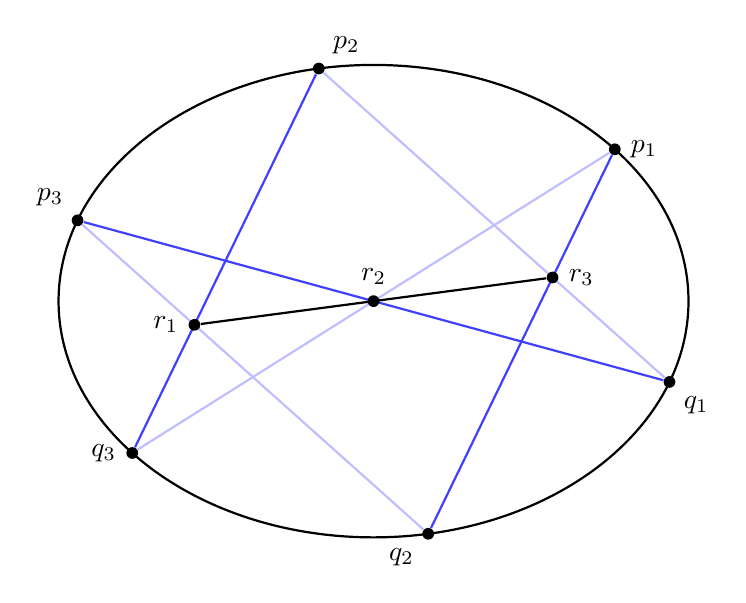
\begin{tikzpicture}
\draw[thick] (0,0) ellipse (4cm and 3cm);
\node[circle,fill,inner sep=1.5pt,label=above left:$p_3$] (p3) at ({4*cos(160)}, {3*sin(160)}) {};
\node[circle,fill,inner sep=1.5pt,label=above right:$p_2$] (p2) at ({4*cos(100)}, {3*sin(100)}) {};
\node[circle,fill,inner sep=1.5pt,label=right:$p_1$] (p1) at ({4*cos(40)}, {3*sin(40)}) {};
\node[circle,fill,inner sep=1.5pt,label=below right:$q_1$] (q1) at ({4*cos(-20)}, {3*sin(-20)}) {};
\node[circle,fill,inner sep=1.5pt,label=below left:$q_2$] (q2) at ({4*cos(-80)}, {3*sin(-80)}) {};
\node[circle,fill,inner sep=1.5pt,label=left:$q_3$] (q3) at ({4*cos(-140)}, {3*sin(-140)}) {};

\draw[thick,blue!75,name path=l23] (p2) -- (q3);
\draw[thick,blue!25,name path=l32] (p3) -- (q2);
\draw[thick,blue!25,name path=l13] (p1) -- (q3);
\draw[thick,blue!75,name path=l31] (p3) -- (q1);
\draw[thick,blue!75,name path=l12] (p1) -- (q2);
\draw[thick,blue!25,name path=l21] (p2) -- (q1);

\path [name intersections={of=l23 and l32, by=r1}];
\path [name intersections={of=l13 and l31, by=r2}];
\path [name intersections={of=l12 and l21, by=r3}];
\node[circle,fill,inner sep=1.5pt,label=left:$r_1$] (r1) at (r1) {};
\node[circle,fill,inner sep=1.5pt,label=above:$r_2$] (r2) at (r2) {};
\node[circle,fill,inner sep=1.5pt,label=right:$r_3$] (r3) at (r3) {};

\draw[thick] (r1) -- (r3);
\end{tikzpicture}
\end{center}
\end{thm}

\begin{proof}
Consider the two cubics $L_{12}\cup L_{23}\cup L_{31}$ and $L_{21}\cup L_{32}\cup L_{13}$, which intersect at exactly the 9 points $p_1,p_2,p_3,q_1,q_2,q_3,r_1,r_2,r_3$, and the cubic $C\cup L$ where $L$ is the line that goes through $r_1$ and $r_2$, which passes through $p_1,p_2,p_3,q_1,q_2,q_3,r_1,r_2$. Applying Cayley--Bacharach to the three cubics gives us $r_3\in C\cup L$, so it remains to show $r_3\notin C$, but this is trivial: if $r_3\in C$ then $L_{12}\subset C$, but then $C=L_{12}\cup\widetilde C$ is a union of two lines, so there must be three of $p_1,p_2,p_3,q_1,q_2,q_3$ being collinear, contradicting assumption.
\end{proof}

\begin{flushright}
\textit{Week 7, lecture 1, 11th November}
\end{flushright}

\subsection{Resultant, reprise, and a better theorem}

\begin{prop}
\label{prop:explicitresultant}
Let $f,g\in R[x]$ and write $f(x)=a(x-\lambda_1)\cdots(x-\lambda_d)$ and $g(x)=b(x-\mu_1)\cdots(x-\mu_e)$ where $d,e>0$. Then
\[
\re_{f,g}=a^eb^d\prod_{1\leq i\leq d\atop 1\leq j\leq e}(\lambda_i-\mu_j)=a^e\prod_{i=1}^d g(\lambda_i)
\]
\end{prop}
\begin{proof}
First observe that for any arbitrary $f,g\in R[x]$ and $a,b\in R$, one has $\re_{af,bg}=a^eb^d\re_{f,g}$ by the fact that multiplying one row of the matrix $M$ by $\lambda$ changes $\det M$ by a factor of $\lambda$ as well, so it suffices to prove the case where $a=b=1$.

Consider the ring homomorphism
\[
\begin{aligned}
\psi:S:=R[y_1,\ldots,y_d,z_1,\ldots,z_e]&\rightarrow R \\
y_i&\mapsto\lambda_i \\
z_j&\mapsto\mu_j,
\end{aligned}
\]
which extends to a homomorphism $\overline\psi:S[x]\rightarrow R[x]$, under which $\overline f=\prod_{i=1}^d(x-y_i)$ is mapped to $f$ and $\overline g=\prod_{j=1}^e(x-z_j)$ is mapped to $g$. It's then clear that $\psi\left(\re_{\overline f,\overline g}\right)=\re_{f,g}$.

Now if $y_i-z_j=0$, then $(x-y_i)$ and $(x-z_j)$ are common factors of $\overline f,\overline g$, hence $\re_{\overline f,\overline g}=0$ by \ref{defnthm:resultant}. Hence $(y_i-z_j)\mid\re_{\overline f,\overline g}$. Apply this to any pair $i,j$ and compare degrees, one has
\[
\re_{\overline f,\overline g}=c\prod_{1\leq i\leq d\atop 1\leq j\leq e}(y_i-z_j)
\]
for some constant $c$. Substituting $y_i=1,z_j=0$ for all $i,j$, one has $\overline f=(x-1)^d$ and $\overline g=x^e$, so
\[
c=c(1-0)^{de}=\re_{(x-1)^d,x^e}=\det\left(
\begin{array}{c|cccccc}
\ast & (-1)^d & 0 & 0 & \cdots & 0 \\
\ast & \ast & (-1)^d & 0 & \cdots & 0 \\
\ast & \ast & \ast & (-1)^d & \cdots & 0 \\
\vdots & \vdots & \vdots & \vdots & \ddots & \vdots \\
\ast & \ast & \ast & \ast & \cdots & (-1)^d \\ \hline
I_d & 0 & 0 & 0 & \cdots & 0
\end{array}\right),
\]
now, moving the last $d$ row to the top requires $de$ exchanges of two rows, with the resulting matrix with determinant $1^d\cdot \left((-1)^d\right)^e=(-1)^de$, so $(-1)^{de}c=(-1)^de$, i.e. $c=1$.
\end{proof}

\begin{prop}
\label{prop:resoflinearwithgeneral}
If $g\in R[x]$ has $\deg g\geq 1$, then $\re_{x-c,g(x)}=g(c)$.
\end{prop}
\begin{proof}
Applying (the second equality of) \ref{prop:explicitresultant} one has
\[
R_{x-c,g(x)}=\prod_{i=1}^1g(c)=g(c).
\]
But $g$ may not completely split into linear factors, so it remains to show that resultant is invariant in $\overline k$, the algebraic closure of the field of fractions $k$ of $R$, which is clear.
\end{proof}

\begin{prop}
\label{prop:ResfghisResfgplusResfh}
For nonconstant $f,g,h\in R[x],\ \re_{f,gh}=\re_{f,g}\re_{f,h}$.
\end{prop}
\begin{proof}
Use the same trick to consider $f,g,h\in\overline k[x]$ where $\overline k$ is algebraically closed, and write
\[
f(x)=a(x-\lambda_1)\cdots (x-\lambda_d),
\]
then by \ref{prop:explicitresultant}
\[
\re_{f,gh}=a^{\deg gh}\prod_{i=1}^d gh(\lambda_i)=\left(a^{\deg g}\prod_{i=1}^d g(\lambda_i)\right)\left(a^{\deg h}\prod_{i=1}^d h(\lambda_i)\right)=\re_{f,g}\re_{f,h}.
\]
\end{proof}

\begin{prop}
\label{prop:ResfgisResfhgplusg}
For $f,g,h\in R[x]$ such that $f,g,hf+g$ are nonconstant and $f$ is monic, $\re_{f,g}=\re_{f,hf+g}$.
\end{prop}
\begin{proof}
Again applying \ref{prop:explicitresultant} and writing $f=\prod_{i=1}^d(x-\lambda_i)$ one has
\[
\re_{f,g+hf}=\prod_{i=1}^d (hf+g)(\lambda_i)=\prod_{i=1}^d (h(\lambda_i)f(\lambda_i)+g(\lambda_i))=\prod_{i=1}^d g(\lambda_i)=\re_{f,g}.
\]
\end{proof}

\begin{flushright}
\textit{Week 7, lecture 2, 11th November}
\end{flushright}

\begin{remark}
Consider the curves $C:y=x^2-t$ and $D:y=0$. By \ref{thm:weakBezout}, they have at most two intersection points. But when $t=0$, naively they have only one intersection at the origin. This is messy and we want to refine our formation of the theorem so that these exceptions don't appear by associating a number $I_p(C,D)$, intersection multiplicity, for the intersection of $C$ and $D$ at $p$ so that we have the universal form $\sum_{p\in C\cap D}I_p(C,D)=\deg f\cdot \deg g$.

Naively we want $I_p(C,D)$ to satisfy:
\begin{enumerate}
\item $I_p(C,D)=I_p(D,C)$
\item $p\notin C\cap D\implies I_p(C,D)=0$
\item If a curve $C_0\subset C\cap D$ and $p\in C_0$, then $I_p(C,D)=\infty$
\item If $C,D$ are distinct lines intersecting at $p$, then $I_p(C,D)=1$
\item $D=D_1\cap D_2\implies I_p(C,D)=I_p(C,D_1)+I_p(C,D_2)$
\item For $C=\{F=0\}$ and $D=\{G=0\}$, one has $I_p(C,D)=I_p(C,D')$ where $D'=\{FQ+G=0\}$. In English, if I perturb my curve a little bit, the multiplicity shouldn't change
\end{enumerate}
So, how do we uniquely define $I_p(C,D)$ so that it always satisfy the above?
\end{remark}

\begin{example}
By the properties above, for $p=[0,0,1]$,
\[
I_p(y^2z-x^3,x)=I_p(x,y^2z-x^3)=I_p(x,y^2z)=2I_p(x,y)+I_p(x,z)=2,
\]
so from the properties without any explicit formula, one can uniquely determine (at least in this case) $I_p(C,D)$!
\end{example}

\begin{defnthm}
There's one and only one way to define the \textit{intersection multiplicity} $I_p(C,D)$ that satisfies the 6 properties above.
\end{defnthm}
\begin{proof}
For uniqueness, see Frances Kirwan's \textit{Complex algebraic curves}, in which she proved by induction on $k=I_p(C,D)$ (express $I_p(C,D)=k$ by intersection multiplicities strictly less than $k$ by the 6 properties).

We define $I_p(C,D)$ as follows:
\begin{enumerate}
\item If $p\notin C\cap D$ then $I_p(C,D)=0$.
\item If $p$ lies on a common component of $C,D$, then $I_p(C,D)=\infty$.

\item Now consider $C'\subset C$ and $D'\subset D$ such that $C',D'$ have no common components. Observe that in the 6 properties above, we didn't mention any specific coordinates, which means for any projective transformation $\phi$, one has
\[
I_{\phi(p)}(\phi(C'),\phi(D'))=I_p(C',D'),
\]
so WLOG suppose $[1,0,0]\notin\{C',D'\text{ lines through pairs of intersections of }C',D'\}$.

If $\K$ is algebraically closed, recall proof of \ref{thm:weakBezout} and write $C'=\{F=0\},D'=\{G=0\}$ and
\[
\re_{F,G}=\prod_{i=1}^{de}(a_iy+b_iz).
\]
We proved that $\exists x_0\in\K:[x_0,y_0,z_0]\in C\cap D\iff [y_0,z_0]=[-b_i,a_i]$ for some $i$, and such $x_0$ is unique. Moreover, every intersection corresponds to one such $x_0$.

Then, write $p=[a,b,c]$ and define $I_p(C,D)$ as the usual multiplicity of $[b,c]$ as a root of $\re_{F,G}(y,z)$, i.e. the largest $k$ such that $(cy-bz)^k\mid\re_{F,G}(y,z)$.
\end{enumerate}

\begin{flushright}
\textit{Week 7, lecture 3, 15th November}
\end{flushright}

It remains to check this definition satisfies the 6 properties.

\begin{enumerate}
\item This is clear since $R_{F,G}(y,z)=\pm R_{G,F}(y,z)$, so their roots are exactly the same.
\item By definition.
\item By definition.
\item Write $\ell_1=\{f_1(x)=ax+by+cz=0\}$ and $\ell_2=\{f_2(x)=dx+ey+fz=0\}$, then
\[
p=[bf-ce,cd-af,ae-bd].
\]
Since $(a,b,c)\neq (d,e,f)$, indeed $p\in\p^2(\K)$. By applying a projective transformation, we can assume $p\neq [1,0,0]$ and write
\[
R_{f_1,f_2}=\det\begin{pmatrix}
a & by+cz \\ d & ey+fz
\end{pmatrix}=(ae-bd)y+(af-cd)z,
\]
and clearly the root $[cd-af,ae-bd]$ has multiplicity 1. 
\item By \ref{prop:ResfghisResfgplusResfh}.
\item By \ref{prop:ResfgisResfhgplusg}.
\end{enumerate}
\end{proof}

\begin{thm}[Bézout]
\label{thm:strongBezout}
If $\K$ is algebraically closed and $C,D\subset\p^2(\K)$ are two curves of degree $d,e\geq 1$ with no common component, then
\[
\sum_{p\cap D}I_p(C,D)=de.
\]
\end{thm}
\begin{proof}
Repeat the proof $\ref{thm:weakBezout}$ and apply the definition above.
\end{proof}

\begin{defn}
$C,D\subset\p^2(\K)$ are \textit{transverse} at $p\in C\cap D$ if $p$ is smooth on both curves and $I_p(C,D)=1$.
\end{defn}
Then, \ref{thm:strongBezout} says two smooth curves $C,D$ has $\deg C\deg D$ intersections $\iff C,D$ intersect transversely at every intersection.

\begin{prop}
\label{prop:transviffTpCdiffTpD}
$C,D$ are transverse at $p\iff T_pC\neq T_pD$.
\end{prop}
\begin{proof}
Since $p$ is smooth, there is a unique irreducible component $C'$ of $C$ that passes through $p$ by \ref{prop:nodesaresingular}, and since $I_p(C,D)=I_p(C',D)$, one can assume $C$, and symmetrically $D$ are irreducible. Moreover $C$ and $D$ can be assumed to be different since if $C=D$ then $I_p(C,D)=\infty$ and of course $T_pC=T_pD$. WLOG suppose $\deg C=d\geq e=\deg D$.

By \ref{thm:weakBezout}, $|C\cap D|<\infty$. Apply a projective transformation so that $p=[0,0,1],\ T_pD=\{x=0\}$ and none of $C,D$ or lines through pairs of intersections of $C$ and $D$ passes through $[1,0,0]$. Now we can write $I_p(C,D)$ using resultants. Write $F(x,y,z)=f_0(y,z)x^d+\cdots+f_d(y,z)$ and $G(x,y,z)=g_0(y,z)x^e+\cdots+g_e(y,z)$ where $f_i,g_i$ are homogeneous of degree $i$. Then $I_p(C,D)$ is the largest $k$ such that $y^k\mid\re_{F,G}(y,z)$.

By \ref{prop:eulersid}, $0=dF(0,0,1)=\frac{\partial F}{\partial z}(0,0,1)$, so since $p$ is smooth, $\left(\frac{\partial F}{\partial x}(0,0,1),\frac{\partial F}{\partial y}(0,0,1)\right)\neq (0,0)$. Now write $f_d(y,z)=az^d+bz^{d-1}y+\cdots$ where $y^2\mid\cdots$. Note that $F(0,0,1)=0=f_d(0,1)=a$, and $b=\frac{\partial F}{\partial y}(0,0,1)$. Hence $y^2\mid f_d(y,z)\iff b=0\iff T_pC=\{x=0\}=T_pD$.

\begin{flushright}
\textit{Week 8, lecture 1, 18th November}
\end{flushright}

Via the same argument, $T_pC=T_pD\iff y^2\mid g_e(y,z)$. Also, since $g_{e-1}(0,1)=\frac{\partial G}{\partial x}(0,0,1)\neq 0$, one can rescale and assume $g_{e-1}(0,1)=1$. Now if $e=1$, then $G(x,y,z)=g_e(y,z)+x$, so $T_pC=T_pD\iff G(x,y,z)=x$. By \ref{prop:resoflinearwithgeneral}, we then have (up to sign) $\re_{F,G}=F(0,y,z)=f_d(y,z)$, so we're done.

If $e\geq 2$,
\[
\re_{F,G}=\det\begin{pmatrix}
f_0 & \cdots & f_d \\
& f_0 & \cdots & f_d \\
& & \ddots & & \ddots \\
& & & f_0 & \cdots & f_d \\
g_0 & \cdots & g_e \\
& g_0 & \cdots & g_e \\
& & \ddots & & \ddots \\
& & & g_0 & \cdots & g_e \\
\end{pmatrix}
\]
but if one looks at the last column, one can write it in the form $\re_{F,G}=\pm f_d\det A\pm g_e\det B$ for some minors $A,B$, hence it remains to prove that $T_pC\neq T_pD\implies y^2\nmid\re_{F,G}(y,z)$. Let's be a bit more careful and write
\[
\re_{F,G}\equiv f_d\det\begin{pmatrix}
f_0 & \cdots & f_d \\
& f_0 & \cdots & f_d \\
& & \ddots & & \ddots \\
& & & f_0 & \cdots & f_d \\
g_0 & \cdots & g_{e-1} & 0 \\
& g_0 & \cdots & g_{e-1} & 0 \\
& & \ddots & & \ddots \\
& & & g_0 & \cdots & g_{e-1} \\
\end{pmatrix}\equiv \re_{F,H}(y,z)\Mod y^2
\]
where
\[
H(x,y,z)=g_0(y,z)x^{e-1}+\cdots+g_1(y,z)x^{e-1}+\cdots+g_{e-2}(y,z)x+g_{e-1}(y,z),
\]
so $G=Hx+g_e$, hence if we can show $y\nmid \re_{F,H}$ then $y^2\nmid\re_{F_G}$. Suppose for a contradiction that $y\mid \re_{F,H}$, then $[0,1]$ is a root so $\{F=0\}$ and $\{H=0\}$ intersect at $[\lambda,0,1]$ for some $\lambda$. If $\lambda=0$ then $H(0,0,1)=g_{e-1}(0,1)=0$, a contradiction. If $\lambda\neq 0$, $G(\lambda,0,1)=H(\lambda,0,1)\lambda+g_e(0,1)=0$ since $g_e(0,1)=G(0,0,1)=0$. But then the line through $[\lambda,0,1]$ and $[0,0,1]$ passes through $[1,0,0]$, a contradiction.
\end{proof}

\begin{coro}
\label{coro:IpCLgeq2iffLisTpC}
For a smooth point $p\in C\subset\p^2$ and a line $L$, one has $I_p(C,L)\geq 2\iff L=T_p(C)$.
\end{coro}

\begin{flushright}
\textit{Week 8, lecture 2, 18th November}
\end{flushright}

\begin{notation}
For $\alpha=(\alpha_1,\alpha_2,\alpha_3)$ where $\alpha_i\in\N$, write $|\alpha|:=\alpha_1+\alpha_2+\alpha_3$ and
\[
\partial^\alpha F:=\frac{\partial^{|\alpha|}F}{\partial x^{\alpha_1}\partial y^{\alpha_2}\partial z^{\alpha_3}}.
\]
\end{notation}
\begin{defn}
$p=[a,b,c]\in C=\{F=0\}$ has \textit{multiplicity} $m_p(C)=k$ if
\begin{enumerate}
\item all $\left.\partial^\alpha F\right|_p=0$ for $|\alpha|<k$ and
\item $\left.\partial^\alpha F\right|_p\neq 0$ for some $\alpha$ with $|\alpha|=k$.
\end{enumerate}
\end{defn}
This doesn't depend on the coordinates $a,b,c$ since $\partial^\alpha F$ is homogeneous of degree $\deg F-|\alpha|$ if $F$ is homogeneous.

\begin{remark}
Note that
\begin{enumerate}
\item $p$ is smooth $\iff m_p(C)=1$.
\item $m_p(C)=m_{\phi(p)}(\phi(C))$ for any projective transformation $\phi$.
\item $m_p(C)\leq \deg C$.
\item If $p\in C$ and $p\notin D$, then $m_p(C)=m_p(C\cup D)$, i.e. multiplicity is a local behaviour (by product rule)
\end{enumerate}
\end{remark}

\begin{example}
The point $p=[0,0,1]$ on $C=\{F(x,y,z)=y^2z-x^3=0\}$ is singular, but how singular is it? Note that
\[
\partial^{(0,2,0)}F|_{[0,0,1]}=\frac{\partial^2F}{\partial y^2}|_{[0,0,1]}=2\neq 0,
\]
so $m_p(C)=2$, so not \textit{that} singular.
\end{example}

\begin{prop}
Let $\K$ be of character zero and $C,D\subset\p^2(\K)$ with $p\in C\cap D$. Then $I_p(C,D)\geq m_p(C)m_p(D)$.
\end{prop}
\begin{proof}
If $C$ and $D$ have a common component, then $I_p(C,D)=\infty$ so there's nothing to prove, so assume $C$ and $D$ have no common components. Write $r:=m_p(C)$ and $s=m_p(D)$. As always, apply a projective transformation such that $p=[0,0,1]$ and the point $[1,0,0]\notin\{C,D,\text{ all lines that pass through pairs of points in }C\cap D\}$ and write
\[
F(x,y,z)=f_0(y,z)x^d+\cdots+f_{d-1}(y,z)x+f_d(y,z).
\]
We claim that for any $i=0,\ldots,r$, one has $y^{r-i}\mid f_{d-i}(y,z)$. By definition, $\partial^{(i,j,0)}F|_{p=[0,0,1]}=0 \ \forall i=0,\ldots,r-1$ and $j<r-i$. We now calculate
\[
\frac{\partial^i F}{\partial x^i}=\frac{\partial^i }{\partial x^i}(\cdots)+\frac{\partial^i}{\partial x^i} f_{d-i}x^i+\frac{\partial^i}{\partial x^i} f_{d-i+1}x^{i-1}+\cdots=\frac{\partial^i }{\partial x^i}(\cdots)+i!f_{d-i}
\]
where $\cdots$ are the first $i-1$ terms, but now
\[
0=\partial^{(i,j,0)}F|_{[0,0,1]}=\left.\frac{\partial^j}{\partial y^j}\frac{\partial^i }{\partial x^i}(\cdots)\right|_{[0,0,1]}+i!\frac{\partial^j f_{d-i}(0,1)}{\partial y^j}=i!\frac{\partial^j f_{d-i}(0,1)}{\partial y^j},
\]
so if one writes $f_{d-i}=a_0z^{d-i}+a_1yz^{d-i-1}+\cdots$, then in particular for $j=0,\ f_{d-i}(0,1)=0=a_0$, and for $j=1,\ \frac{\partial f_{d-i}}{\partial y}(0,1)=0=a_1$, and one can do this for all $j<r-i$ by above, hence the claim is proven.

Now for any $i\leq r$, write $f_{d-i}(y,z)=y^{r-i}\widetilde f_{d-i}(y,z)$ for some other homogeneous polynomial $\widetilde f$. By the same argument, for any $j\leq s$, one can write $g_{e-j}(y,z)=y^{e-j}\widetilde g_{e-j}(y,z)$. So
\[
\re_{F,G}=\det\begin{pmatrix}
f_0 & \cdots & y^{r-1}\widetilde f_{d-1} & y^r\widetilde f_d \\
& \ddots & & \ddots & \ddots \\
& & f_0 & \cdots & y^{r-1}\widetilde f_{d-1} & y^r\widetilde f_d \\
g_0 & \cdots & y^{s-1}\widetilde g_{e-1} & y^s\widetilde g_e \\
& \ddots & & \ddots & \ddots \\
& & g_0 & \cdots & y^{s-1}\widetilde g_{e-1} & y^s\widetilde g_e
\end{pmatrix}
\]
Now multiplying the last $s$ rows $e,e-1,\ldots,e-s+1$ in the first block by $y^s,y^{s-1},\ldots,y$ respectively and multiplying the last $r$ rows $d+e,d+e-1,\ldots,d+e-r+1$ in the second block by $y^r,y^{r-1},\ldots,y$ respectively changes the determinant to
\[
y^{s+s-1+\cdots+1+r+r-1+\cdots+1}\re_{F,G}=y^{\frac{s(s+1)}{2}+\frac{r(r+1)}{2}}\re_{F,G},
\]
but now the last $r+s$ columns of the new matrix are divisible by $y^{r+s},y^{r+s-1},\ldots,y$ respectively, so the above calculated determinant is divisible by $y^{r+s}y^{r+s-1}\cdots y=y^{\frac{(r+s)(r+s+1)}{2}}$, and since
\[
\frac{(r+s)(r+s+1)}{2}-\frac{s(s+1)}{2}-\frac{r(r+1)}{2}=\frac{r^2+2rs+r+s^2+s-s^2-s-r^2-r}{2}=\frac{2rs}{2}=rs,
\]
one has $y^{rs}\mid\re_{F,G}$.
\end{proof}

\begin{coro}
For $p\in C\cap D$ where $C,D\subset\p^2(\K),\ I_p(C,D)=1\iff p$ is a smooth point of $C$ and $D$ and $T_pC\neq T_pD$.
\end{coro}
\begin{proof}
$I_p(C,D)=1\implies m_p(C)m_p(D)\leq 1\implies m_p(C)=m_p(D)\implies C,D$ are smooth at $p$. It then follows from \ref{prop:transviffTpCdiffTpD}.
\end{proof}

\begin{flushright}
\textit{Week 8, lecture 3, 22nd November: cancelled}
\end{flushright}

\begin{flushright}
\textit{Week 9, lecture 1, 25th November}
\end{flushright}

\begin{coro}
Let $C,D\subset\p^2$ be curves with no common component. Then $C\cap D$ contains exactly $\deg C\deg D$ points $\iff\forall p\in C\cap D$, both $C$ and $D$ are smooth at $p$ and $T_pC\neq T_pD$.
\end{coro}

\begin{prop}
Let $\{F=0\}=C\subset\p^2(\K)$ with degree $d\geq 2$. If $C$ has singular points $p_1,\ldots,p_k$ with multiplicities $r_1,\ldots,r_k$, then $\sum_{i=1}^k r_i(r_i-1)\leq d(d-1)$.
\end{prop}
\begin{proof}
One can write $\{p_1,\ldots,p_k\}=C\cap\left\{\frac{\partial F}{\partial x}=0\right\}\cap\left\{\frac{\partial F}{\partial y}=0\right\}\cap\left\{\frac{\partial F}{\partial z}=0\right\}$. At least one of $\frac{\partial F}{\partial x_i}$ is not constantly zero, so WLOG assume this is $\frac{\partial F}{\partial x}$ is homogeneous of degree $d-1$. Then
\[
\sum_{i=1}^k r_i(r_i-1)\leq \sum_{i=1}^k I_{p_i}\left(C,\left\{\frac{\partial F}{\partial x}=0\right\}\right)\leq \sum_{p\in C\cap\left\{\frac{\partial F}{\partial x}=0\right\}}\left(C,\left\{\frac{\partial F}{\partial x}=0\right\}\right)=d(d-1),
\]
where $m_{p_i}\left(\left\{\frac{\partial F}{\partial x}=0\right\}\right)\geq r_i-1$ follows by definition from the fact that $\partial^k\frac{\partial F}{\partial x}=\partial^{k'}F=0$ where $|k'|=|k|+1$ for all $|k|<r_i-1$ (i.e. $|k'|<r_i$).
\end{proof}

\begin{remark}
Since if $p$ is singular then $m_p(C)\geq 2$, we have $\sum_{i=1}^k 2(2-1)=2k\leq d(d-1)$, i.e. the number of singularities of a curve of degree $d$ is bounded above by $\frac{d(d-1)}{2}=\binom{d}{2}$.

Can we have a curve of degree $d$ with exactly $\binom{d}{2}$ singularities? i.e. is our upper bound sharp? Consider the curve $C=\bigcup_{i=1}^d L_i$ where no three $L_i$'s intersect at the same point, then singularities of $C$ are exactly the $\binom{d}{2}$ intersections of $L_i$'s.
\end{remark}

\subsection{Classification of cubic curves}
We have seen that \hyperref[thm:irredconicsaresmooth]{irreducible conics are smooth} as an application of the weak Bézout theorem, now let's classify cubics with the strong one.

\begin{lemma}
If an irreducible cubic $C\subset\p^2(\K)$ is not smooth, then it has exactly one singularity of multiplicity 2 (a \textit{double point}).
\end{lemma}
\begin{proof}
Let $p$ be a singularity and $q$ any other point of $C$, and let $L$ be the unique line through $p$ and $q$. Then
\[
m_q(C)+2\leq m_q(C)+m_p(C)\leq I_q(C,L)+I_p(C,L)\leq\sum_{r\in C\cap L}I_r(C,L)=\deg C\deg L=3,
\]
so $m_q(C)=1$, i.e. $q$ is smooth, and we have $m_p(C)=2$.
\end{proof}

\begin{flushright}
\textit{Week 9, lecture 2, 25th November}
\end{flushright}

\begin{defn}
Let $C=\{F=0\}\subset\p^2(\K)$ be a smooth curve of degree $d\geq 1$. The \textit{Hessian matrix} of $F$ is
\[
\begin{pmatrix}
\frac{\partial^2 F}{\partial x^2} & \frac{\partial^2 F}{\partial x\partial y} & \frac{\partial^2 F}{\partial x\partial z} \\
\frac{\partial^2 F}{\partial y\partial x} & \frac{\partial^2 F}{\partial y^2} & \frac{\partial^2 F}{\partial y\partial z} \\
\frac{\partial^2 F}{\partial z\partial x} & \frac{\partial^2 F}{\partial z\partial y} & \frac{\partial^2 F}{\partial z^2},
\end{pmatrix}
\]
and the \textit{Hessian} of $F$, denoted by $H_F$, is the determinant of the Hessian matrix, which has degree $3(d-2)$.
\end{defn}

\begin{defn}
A smooth $p\in C$ is an \textit{inflection point} if $H_F(p)=0$, i.e. inflection points are precisely $\{F=0\}\cap\{H_F=0\}$, which is nonempty if $d\geq 3$.
\end{defn}

Let's first simplify the calculation of the Hessian using \ref{prop:eulersid}:

\begin{lemma}
If $F\in\K[x,y,z]$ is homogeneous of degree $d\geq 2$, then
\[
z^2H_F(x,y,z)=(d-1)^2\det\begin{pmatrix}
\frac{\partial^2 F}{\partial x^2} & \frac{\partial^2 F}{\partial x\partial y} & \frac{\partial F}{\partial x} \\
\frac{\partial^2 F}{\partial y\partial x} & \frac{\partial^2 F}{\partial y^2} & \frac{\partial F}{\partial y} \\
\frac{\partial F}{\partial x} & \frac{\partial F}{\partial y} & \frac{d}{d-1}F
\end{pmatrix},
\]
and similarly for $x$ and $y$.
\end{lemma}
\begin{proof}
Note that
\[
\begin{aligned}
zH_F&=\det \begin{pmatrix}
\frac{\partial^2 F}{\partial x^2} & \frac{\partial^2 F}{\partial x\partial y} & z\frac{\partial^2 F}{\partial x\partial z} \\
\frac{\partial^2 F}{\partial y\partial x} & \frac{\partial^2 F}{\partial y^2} & z\frac{\partial^2 F}{\partial y\partial z} \\
\frac{\partial^2 F}{\partial z\partial x} & \frac{\partial^2 F}{\partial z\partial y} & z\frac{\partial^2 F}{\partial z^2}
\end{pmatrix}=\det \begin{pmatrix}
\frac{\partial^2 F}{\partial x^2} & \frac{\partial^2 F}{\partial x\partial y} & z\frac{\partial^2 F}{\partial x\partial z}+x\frac{\partial^2 F}{\partial x^2}+y\frac{\partial^2 F}{\partial x\partial y} \\
\frac{\partial^2 F}{\partial y\partial x} & \frac{\partial^2 F}{\partial y^2} & z\frac{\partial^2 F}{\partial y\partial z}+x\frac{\partial^2 F}{\partial y\partial x}+y\frac{\partial^2 F}{\partial y^2} \\
\frac{\partial^2 F}{\partial z\partial x} & \frac{\partial^2 F}{\partial z\partial y} & z\frac{\partial^2 F}{\partial z^2}+x\frac{\partial^2 F}{\partial z\partial x}+y\frac{\partial^2 F}{\partial z\partial y}
\end{pmatrix} \\
&=\det \begin{pmatrix}
\frac{\partial^2 F}{\partial x^2} & \frac{\partial^2 F}{\partial x\partial y} & (d-1)\frac{\partial F}{\partial x} \\
\frac{\partial^2 F}{\partial y\partial x} & \frac{\partial^2 F}{\partial y^2} & (d-1)\frac{\partial F}{\partial y} \\
\frac{\partial^2 F}{\partial z\partial x} & \frac{\partial^2 F}{\partial z\partial y} & (d-1)\frac{\partial F}{\partial z}
\end{pmatrix}=(d-1)\det \begin{pmatrix}
\frac{\partial^2 F}{\partial x^2} & \frac{\partial^2 F}{\partial x\partial y} & \frac{\partial F}{\partial x} \\
\frac{\partial^2 F}{\partial y\partial x} & \frac{\partial^2 F}{\partial y^2} & \frac{\partial F}{\partial y} \\
\frac{\partial^2 F}{\partial z\partial x} & \frac{\partial^2 F}{\partial z\partial y} & \frac{\partial F}{\partial z}
\end{pmatrix},
\end{aligned}
\]
and we repeat the operation for the 3rd row again.
\end{proof}

\begin{prop}
A smooth point $p\in C$ is an inflection point $\iff I_p(C,T_pC)\geq 3$.
\end{prop}
\begin{proof}
Since the Hessian and intersection multiplicities are invariant under projective transformation, suppose $[1,0,0]\notin C,\ p=[0,0,1]$ and $T_pC=\{x=0\}$. Write
\[
F(x,y,z)=x^df_0(y,z)+x^{d-1}f_1(y,z)+\cdots+xf_{d-1}(y,z)+f_d(y,z)\qquad\text{where }f_i\text{ is homogeneous of degree }i,
\]
then $I_p(C,T_pC)$ is the largest $k$ such that $y^k\mid\re_{x,F}=F(0,y,z)=f_d(y,z)$ by \ref{prop:resoflinearwithgeneral}, so
\[
I_p(C,T_pC)\geq 3\iff y^3\mid f_d(y,z).
\]
We now claim $y^3\mid f_d(y,z)\iff\frac{\partial^2 F}{\partial y^2}(0,0,1)=0$. Indeed, $\frac{\partial^2 F}{\partial y^2}(0,0,1)=\frac{\partial^2 f_d}{\partial y^2}(0,1)$ since when taking derivatives with respect to $y$, all $x$'s are preserved. Now write
\[
f_d(y,z)=a_0z^d+a_1z^{d-1}y+a_2z^{d-2}y^2+y^3(\cdots),
\]
which is divisible by $y^3\iff a_0=a_1=a_2=0$. But $a_0=F(0,0,1)$ and we assumed $[0,0,1]=p\in C$, and $a_1=\frac{\partial F}{\partial y}(0,0,1)=0$ since $T_pC=\{x=0\}$, so $y^3\mid f_d(y,z)\iff a_2=\frac{\partial^2 f_d}{\partial y^2}(0,1)=0$. Then
\[
\frac{z^2}{(d-1)^2}H_F(0,0,1)=\det\begin{pmatrix}
\frac{\partial^2 F}{\partial x^2} & \frac{\partial^2 F}{\partial x\partial y} & \frac{\partial F}{\partial x} \\
\frac{\partial^2 F}{\partial y\partial x} & 0 & 0 \\
\frac{\partial F}{\partial x} & 0 & 0
\end{pmatrix}=0,
\]
\end{proof}

\begin{flushright}
\textit{Week 9, lecture 3, 29th November: problem class}
\end{flushright}

\begin{flushright}
\textit{Week 10, lecture 1, 2nd December}
\end{flushright}

\section{Riemann surfaces}
\subsection{Definitions and holomorphic functions}
\begin{defn}
A \textit{surface} is a Hausdorff space $S$ with a \textit{countable atlas} $\{(U_i,\phi_i)\}_{i\in I}$ such that
\begin{enumerate}
\item $U_i\subset S$ are open subsets and $\bigcup_{i\in I}U_i=S$ (i.e. $U_i$ form an open cover of $S$),
\item each $\phi_i:U_i\rightarrow V_i$ is a homeomorphism onto an open subset $V_i\subset\C=\R^2$, and
\item $\forall i,j\in I,$ the \textit{transition map} $\phi_i(U_i\cap U_j)\xrightarrow{\phi_j\circ\phi_i^{-1}} \phi_j(U_i\cap U_j)$ is continuous. In plain English, if a point is in the intersection of two different sets of the open cover, then its two images in $\R^2$ are compatible. This gives us the chance to understand the topological space via the Euclidean space $\R^2$.
\end{enumerate}
\end{defn}

\begin{defn}
$S$ is a \textit{Riemann surface} if $\forall i,j\in I$, the transition map $\phi_j\circ\phi_i^{-1}$ is holomorphic, i.e. complex differentiable, or equivalently if one writes $f(x+yi)=\Re(x,y)+i\Im(x,y)$ where $\Re,\Im:\R^2\rightarrow \R$, then $\Re,\Im$ are infinitely differentiable and satisfy the Cauchy--Riemann equations.
\end{defn}

\begin{example}
\label{example:P1CasRiemannsurf}
$\p^1(\C)$ is an example of a Riemann surface and called the \textit{Riemann sphere}. One can define $U_0=\{[x,y]\in\p^1:x\neq 0\}$ and $U_1=\{[x,y]\in\p^1:y\neq 0\}$, with $\phi_0:[x,y]\mapsto\frac{y}{x}$ and $\phi_1:[x,y]\mapsto\frac{x}{y}$. Clearly $U_0\cup U_1=\p^1(\C)$ and $\phi_0,\phi_1$ are homeomorphisms. Now $\phi_1\circ\phi_0^{-1}:\phi_0(U_0\cap U_1)\rightarrow\phi_1(U_0\cap U_1):\C\backslash\{0\}\rightarrow\C\backslash\{0\}$ is given by $z\mapsto[1,z]\mapsto\frac{1}{z}$, which is holomorphic.
\end{example}

\begin{example}[Complex torus]
Pick $\omega_1,\omega_2\in\C$ such that $\frac{\omega_1}{\omega_2}\notin\R$ and consider the lattice
\[
\Lambda=\{m\omega_1+n\omega_2:m,n\in\Z\}
\]
and the quotient $\C/\Lambda$ with the natural quotient map $\pi:\C\rightarrow\C/\Lambda$. Now imagine $\omega_1,\omega_2$ as two vectors in different directions forming a parallelogram, which represents $C/\Lambda$. But the two pairs of opposite sides are equivalent as well (with differences $\omega_1,\omega_2\in\Lambda$), so one can ``glue'' one pair first to form a cylinder, and then glue the two ends to form a torus.

We now claim $C/\Lambda$ is a Riemann surface. Fix $z\in\C/\Lambda$ and $z_0\in\pi^{-1}(z)$. Let $V\subset\C$ be an open ball of radius $\varepsilon$ around $z_0$ such that $\left.\pi\right|_{V}:V\rightarrow\C/\Lambda$ is homeomorphic onto its image. Call its image $U$ and let $\phi=\left(\left.\pi\right|_V\right)^{-1}$. Then for each point $z\in\C/\Lambda$ we obtain a pair $(U,\phi)$. To see this gives countable atlas, it remains to see that $S$ is compact so any open cover has a finite subcover.

Now two different $U$'s differ only by our choice of $z_0$, but they differ by some $c\in\Lambda$, so each transition map is just a translation by an element in the lattice.
\end{example}

\begin{thm}
\label{thm:smoothcurvesareRiemsurf}
Any smooth plane curve $C\subset\p^2(\C)$ is a Riemann surface.
\end{thm}

To prove this, recall
\begin{thm}[Holomorphic implicit function theorem]
Let $f:\C^2\rightarrow\C$ be a holomorphic function. If $(a,b)\in\C^2$ satisfies $f(a,b)=0$ and $\frac{\partial f}{\partial y}(a,b)\neq 0$, then there is an open neighbourhood $\Omega\subset\C$ of $a$ and a holomorphic function $g:\Omega\rightarrow\C$ such that $g(a)=b$ and the graph $\{(x,g(x):x\in\Omega)\}$ of $g$ is precisely the zero set of $f^{-1}(0)$ over some open neighbourhood of $(a,b)$.
\end{thm}

\begin{flushright}
\textit{Week 10, lecture 2, 2nd December}
\end{flushright}

\begin{proof}[Proof of \ref{thm:smoothcurvesareRiemsurf}]
Write $C=\{F=0\}$ where $F$ is irreducible. Pick a point $C\ni p=[a,b,c]$ where $c\neq 0$ and consider the chart $\{z=1\}\subset\p^2(\C)$. Then $C\cap \{z=1\}=\{F(x,y,1)=:f(x,y)=0\}$. Since $C$ is smooth, at least one of $f$'s derivatives is nonzero, so suppose it's $y$ and we can apply the implicit function theorem to $f$ and the point $\left(\frac{a}{c},\frac{b}{c}\right)$, which says there is an open neighbourhood $V\subset\C$ of $\frac{a}{c}$ and a holomorphic function $g:V\rightarrow\C$ such that $C\cap W=\{(x,g(x)):x\in V\}$ for some open neighbourhood $W$ of $p$.

Now let $U=C\cap W$ and $\phi:U\rightarrow C:(x,y)\mapsto x$. Then $U$ is an open cover of $C$, and by \ref{remark:PnCiscompact}, there is a finite subcover, so we have a countable atlas.

If along another $\widetilde U\subset\C^2$ one has also $\frac{\partial f}{\partial y}\neq 0$, then the transition map is the identity. But if we can only use $\frac{\partial f}{\partial x}\neq 0$, then by the implicit function theorem, $\widetilde U=\{(h(y),y):y\in\widetilde V\}$ with $\widetilde\phi:(h(y),y)\rightarrow y$, so we have
\[
\begin{aligned}
\phi(U\cap \widetilde U)\xrightarrow{\phi^{-1}}&U\cap\widetilde U\xrightarrow{\widetilde\phi}\widetilde\phi(U\cap\widetilde U) \\
x\mapsto & (x,g(x))\mapsto g(x),
\end{aligned}
\]
hence the transition map is $g$, which is holomorphic by construction.
\end{proof}

\begin{remark}
The proof only uses local smoothness, and since by Bézout one has that $C$ has finitely many singular points, $C\backslash\sing C$ is still a Riemann surface.
\end{remark}

\begin{defn}
A function $f:S\rightarrow\C$ where $S$ is a Riemann surface is \textit{holomorphic} if for any atlas
\[
\{(U_i,\phi_i:U_i\rightarrow V_i)\}_{i\in I},
\]
the composition $V_i\xrightarrow{\phi_i^{-1}}U_i\xrightarrow{f}\C$ is holomorphic $\forall i\in I$. This implies $f$ is continuous.
\end{defn}

\begin{prop}[The above is not a very useful notion!]
If $S$ is a compact, connected Riemann surface, then any holomorphic $f:S\rightarrow\C$ is constant.
\end{prop}

\begin{proof}
Recall from complex analysis the maximum modulus principle: let $f:\C\rightarrow\C$ be a holomorphic function on a connected, open domain $D\subset\C$. If $f$ is not constant, then $|f(z)|$ cannot achieve its maximum at an interior point of $D$.

Now for a contradiction suppose $f$ is not constant. Then $|f|:S\rightarrow\R$ achieves its maximum at some $p\in S$ since $S$ is compact. Pass $p$ to a chart $U$ with $\phi:U\rightarrow V$ and consider $V\xrightarrow{f\circ\phi^{-1}}\C$, which by definition is holomorphic. But $|f\circ\phi^{-1}|$ achieves its maximum at $\phi(p)$, so $f\circ\phi^{-1}$ must be constant along $V$.

Finally, let $c=f(p)$, then $f^{-1}(c)$ is closed, but it's also open since $f$ is constant around $p$, so since $S$ is connected, $f^{-1}(C)$ is the whole $S$.
\end{proof}

We've reached a kind of a dead end, but we can: (i) generalise the notion of holomorphic maps to between two Riemann surfaces, and (ii) relax our definition to a weaker one, namely a meromorphic function $f:S\rightarrow\C$.

\begin{defn}
Let $S,S'$ be Riemann surfaces with atlas $\{(U_i,\phi_i:U_i\rightarrow V_i)\}$ and $\{(W_i,\psi_i:W_i\rightarrow X_i)\}$ respectively. A function $f:S\rightarrow S'$ is \textit{holomorphic} if $V_i\xrightarrow{\psi_j\circ f\circ\phi_i^{-1}}X_j$ is holomorphic $\forall i,j$.
\end{defn}

\begin{example}
If $C\subset\p^2(\C)$ is a smooth plane curve with $[0,0,1]\notin C$, then $f:C\rightarrow\p^1(\C):[x,y,z]\mapsto[x,y]$ is holomorphic. (Proof is left as an exercise.)

Also verify that composition of two holomorphic functions is holomorphic.
\end{example}

\begin{flushright}
\textit{Week 10, lecture 3, 6th December}
\end{flushright}

\subsection{Meromorphic functions}
Let $f:U\rightarrow\C$ be holomorphic where $U$ is an open subset of $\C$. Then at any point $a\in U$, one can write the power series $f(z)=\sum_{j=0}^\infty c_j(z-a)^j$ which converges on an open neighbourhood of $a$. Then automatically, if $f$ is holomorphic at $a\in U$ and we have the power series $f(z)=\sum_{j=k}^\infty c_j(z-a)^j$ for some $k\geq 1$, then $f$ has a zero of order $k$ at $a$.

Similarly, if $f:U\backslash\{a\}\rightarrow\C$ is holomorphic, then we have a Laurent series $f(z)=\sum_{j=-\infty}^\infty c_j(z-a)^j$ which converges on the punctured neighbourhood $U\backslash\{a\}$ of $a$. Then we say $f$ has a pole of order $k$ at $a$ if $c_j=0$ for each $j<-k$ and $c_{-k}\neq 0$. If $c_j\neq 0$ for infinitely many $j$'s, then $f$ has an \textit{essential singularity} at $a$.

Note that both zeros and poles are isolated, meaning there is a disc around each zero or pole such that there's no other zero or pole in the disc. It suffices to see that there's not an accumulation of zeros, since if not then the derivatives $c_j$ would vanish and $f$ is identically zero.

\begin{defn}
A function $f:U\rightarrow\C\cup\{\infty\}$ where $U\subset\C$ is open is \textit{meromorphic} if $\exists\{a_1,\ldots,a_n\}\subset U$ such that $\left. f\right|_{U\backslash\{a_1,\ldots,a_n\}}$ is holomorphic and $f$ has poles at each $a_i$.

Let $S$ be a Riemann surface with atlas $\{(U_i,\phi_i:U_i\rightarrow V_i)\}$, then a function is meromorphic if each composition $V_i\xrightarrow{\phi_i^{-1}}U_i\xrightarrow{f}\C\}$ is meromorphic.
\end{defn}

\begin{prop}
\label{prop:nonconstmeromorphic}
There are nonconstant meromorphic functions $f:C\rightarrow\C\cup\{\infty\}$ where $C$ is a smooth projective plane curve.
\end{prop}
\begin{proof}
Write $C=\{F(x,y,z)=0\}$ (where $F$ is irreducible and homogeneous). Let $G,H\in\C[x,y,z]$ be any two irreducible (implying $F\nmid H$), relatively prime and homogeneous polynomials of same degree. Then
\[
f(x,y,z)=\frac{G(x,y,z)}{H(x,y,z)}
\]
does not depend on choice of coordinates and $f$ has poles at zeros of $H$, and apart from these points $f$ is holomorphic since it's a rational function. The zeroes of $H$ are not essential singularities of $f$ since when multiplied by $H$, $f$ is holomorphic. Hence $f$ is meromorphic.
\end{proof}

\begin{thm}
There is a bijection between
\[
\left\{f:C\rightarrow\C\cup\{\infty\}\text{ meromorphic}\right\}\leftrightarrow\left\{\widetilde f:C\rightarrow\p^1(\C)\text{ holomorphic other than }\widetilde f\neq [1,0]\right\}
\]
by sending a meromorphic $f$ to
\[
\widetilde f(p)=\left\{
\begin{aligned}
&[f(p),1]\quad &f(p)\in\C \\
&[1,0]\quad &f(p)=\infty .
\end{aligned}
\right.
\]
\end{thm}

\begin{proof}
It (almost) suffices to prove that the $\widetilde f$ defined above is indeed holomorphic, since the bijection is defined in a natural way: for a holomorphic map $\widetilde f:S\rightarrow\p^1(\C):p\mapsto\left[\widetilde f_1(p),\widetilde f_2(p)\right]$, define the map $f:C\rightarrow C\cup\{\infty\}$ by $[x,y]\mapsto\frac{x}{y}$, which is meromorphic by the proof of \ref{prop:nonconstmeromorphic}.

Equip $\p^1(\C)$ with the atlas in \ref{example:P1CasRiemannsurf} and let $a\in C$. Either $f(a)=\infty$ or not. First suppose $f(a)\neq\infty$, then $\exists U\ni a$ such that $\left. f\right|_U\neq\infty$. Then $C$ has an atlas, so consider homeomorphism $\psi:U\rightarrow V$ where $V\subset\C$. Since $\widetilde f(a)=[f(a),1]$, by possibly restricting $U$, we have $\widetilde f(U)\subset U_1$. Then $V\xrightarrow{\psi^{-1}}U\xrightarrow{\widetilde f}\C\xrightarrow{\phi_1}\p^1(\C)$ sends $x$ to $f\left(\psi^{-1}(x)\right)$, which is holomorphic.

Now if $f(a)=\infty$, then $\exists U\ni a$ such that $\left. f\right|_U\neq 0$. The rest is similar.
\end{proof}

\begin{flushright}
\textit{Week 11, lecture 1, 9th December}
\end{flushright}

\subsection{Degree of holomorphic maps}
\begin{prop}
\label{prop:finpreim}
Let $S,S'$ be compact and connected Riemann surfaces and $f:S\rightarrow S'$ be nonconstant and holomorphic. Then $\forall c\in S',\ |f^{-1}(c)|<\infty$.
\end{prop}
\begin{proof}
For a contradiction, suppose $f^{-1}(c)$ is an infinite set. Since $S$ is compact, $f^{-1}(c)$ has a limit point at some $a\in f^{-1}(c)$. Since $f$ is holomorphic, it's continuous, so $f(a)=c$. Passing to atlas $\phi:U\rightarrow V$ where $U$ is an open neighbourhood of $a\in S$ and $\phi':U'\rightarrow V'$ where $U'$ is an open neighbourhood of $f(a)=c\in S'$ and possibly shrinking $U$ and $V$ so that $f(U)\subset U'$, we have the holomorphic map
\[
g:V\xrightarrow{\phi^{-1}} U\xrightarrow{\left. f\right|_U} U'\xrightarrow{\phi'} V',
\]
so $h=g-g(\phi(a))=g-\phi'(c)$ is also holomorphic, but then $\phi(a)$ is a nonisolated zero of $h$, so $h$ is identically zero (by the discussion beginning the previous subsection) and $g$ is constant, so $f$ is constant on $U$. Now let $A$ be the set of limits points of $f^{-1}(c)$. Since $f$ is constant, $A$ is open, but since $f$ is continuous, $A$ is also closed, so $A=S$, hence $f$ is constant on whole of $S$, a contradiction.
\end{proof}

\begin{prop}
\label{prop:zmapstozn}
Let $f:S\rightarrow S'$ be a holomorphic map where $S,S'$ are Riemann surfaces. Let $a\in S$ and write $f(a)=b$. Suppose $f$ is not constant on a neighbourhood of $a$. Then by the atlas and change of coordinates if necessary, one has bijections $\phi:U\rightarrow\D$ (where $\D$ denotes the open unit disk around 0) and $\phi:U'\rightarrow\D$ with $U,U'$ neighbourhoods of $a,b$ respectively and $\phi(a)=\phi'(b)=0$. Shrinking if necessary one can assume $f(U)\subset U'$.

We claim that the function $\phi'\circ f\circ\phi^{-1}:\D\rightarrow\D$ is $z\mapsto z^n$ for some unique $n\geq 1$.
\end{prop}
\begin{proof}
Omitted and nonexaminable.
\end{proof}

\begin{defn}
The \textit{ramification index} of $f$ at $a\in S$ is the unique $n$ above, denoted by $v_f(s)=n$. If $v_f(s)>1$ then $s$ is a \textit{ramification point} of $f$.
\end{defn}

\begin{lemma}
If $f:S\rightarrow S'$ is holomorphic where $S,S'$ are Riemann surfaces, then ramification points of $f$ are isolated.
\end{lemma}
\begin{proof}
Locally at a ramification point, $f$ can be written as $z\mapsto z^n$ where $n>1$, so around this point there's no other ramification points other than the point ($z=0$) itself.
\end{proof}

\begin{prop}
If $f:S\rightarrow S'$ is holomorphic and $S,S'$ are compact, then
\[
d_f:S'\rightarrow\Z_{\geq 0}:s'\mapsto \sum_{s\in f^{-1}(s')}v_f(s)
\]
is locally constant.
\end{prop}
\begin{proof}
By \ref{prop:finpreim} the sum is well defined, and one can write $f^{-1}(s')=\{s_1,\ldots,s_k\}$. Choose disjoint neighbourhoods $U_i\subset S$ of each $s_i$ and $U'\subset S'$ of $s'$ with $\left. f\right|_{U_i}:U_i\rightarrow U'$ can be written as $z\mapsto z^{n_i}$ where $n_i=v_f(s_i)$.

Let $s''$ be close enough to $s'$ such that $f^{-1}(s'')\subset\bigcup_iU_i$ (by continuity), then $s''$ has $n_i$ preimages in $U_i$ with $v_f=1$, so
\[
d_f(s'')=\sum_{i=1}^k\sum_{s\in f^{-1}(s'')\cap U_i} v_f(s)=\sum_{i=1}^k n_i=d_f(s').
\]
\end{proof}

\begin{defn}
Let $f:S\rightarrow S'$ be a holomorphic map between compact and connected Riemann surfaces. Then the \textit{degree} of $f$ is $\deg f=d_f(s')$ for any $s'\in S'$.
\end{defn}

\begin{flushright}
\textit{Week 11, lecture 2, 9th December}
\end{flushright}

\begin{lemma}
Let $f$ be such a map in the definition above. Then for all but finitely many $s'\in S'$, one has $\deg f=\left|f^{-1}(s')\right|$.
\end{lemma}
\begin{proof}
Since ramification points of $f$ are isolated and $S$ is compact, we have finitely many ramification points $s_1,\ldots,s_k$, so if $s'\in S'\backslash\{f(s_1),\ldots,f(s_k)\}$ then
\[
d_f(s')=\sum_{s\in f^{-1}(s')}v_f(s)=\sum_{s\in f^{-1}(s')}1=\left|f^{-1}(s')\right|.
\]
\end{proof}

\begin{prop}
Let $C\subset\p^2(\C)$ be a smooth plane curve of degree $d\geq 2$. If $[0,0,1]\notin C$, then the holomorphic map $f:C\rightarrow\p^1(\C):[x,y,z]\mapsto [x,y]$ has degree $d$.
\end{prop}
\begin{proof}
First note that if $f:S\rightarrow S'$ is nonconstant and holomorphic, then it's surjective by \ref{prop:zmapstozn}. Now $f^{-1}([a,b])$ consists of points of the form $[a,b,c]$ where $c$ is arbitrary, i.e. the line $\{bx-ay=0\}=:L_{[a,b]}$, so $f^{-1}([a,b])=L_{[a,b]}\cap C$. By lemma above, $\deg f=\left|L_{[a,b]}\cap C\right|$ for all but finitely many $[a,b]\in\p^1$.

Now by Bézout, $\deg C=\sum_{p\in L_{[a,b]}\cap C}I_p\left(L_{[a,b]},C\right)$. Write $C=\{F=0\}$. By \ref{coro:IpCLgeq2iffLisTpC}, $I_p\left(L_{[a,b]},C\right)>1$ iff $L_{[a,b]}=T_pC$, i.e. $\left. \frac{\partial F}{\partial z}\right|_{[a,b,c]}=0$, but $\frac{\partial F}{\partial z}$ is not identically zero since if not then $[0,0,1]\in C$, so $I_p\left(L_{[a,b]},C\right)>1$ iff $p\in\left\{\frac{\partial F}{\partial z}=0\right\}\cap C$, so $I_p\left(L_{[a,b]},C\right)=1$ for all but finitely many $[a,b]$, i.e. $\deg C=\left|L_{[a,b]}\cap C\right|$.
\end{proof}

\hrule

\hspace{1mm}

\textbf{Mastery material}: Riemann--Hurwitz formula and genus--degree formula, see lecture notes.

\textbf{Exam}: past papers are available on Blackboard, 70--75\% of questions will be bookwork. Questions 1--4 are for all, question 5 is mastery. Be short and precise, don't overexplain and save time for hard questions.

\end{document}
